\documentclass[12pt]{article}
\usepackage[paper=letterpaper,margin=2cm]{geometry}
\usepackage{amsmath}
\usepackage{amssymb}
\usepackage{amsfonts}
\usepackage{newtxtext, newtxmath}
\usepackage{enumitem}
\usepackage{titling}
\usepackage{multirow}
\usepackage{textcomp}
\usepackage{graphicx}
\usepackage{tikz}
\usepackage{listings}
\usepackage{xcolor}
\graphicspath{ {./images/} }

\definecolor{codegreen}{rgb}{0,0.6,0}
\definecolor{codegray}{rgb}{0.5,0.5,0.5}
\definecolor{codepurple}{rgb}{0.58,0,0.82}
\definecolor{backcolour}{rgb}{0.95,0.95,0.92}

\lstdefinestyle{mystyle}{
    backgroundcolor=\color{backcolour},   
    commentstyle=\color{codegreen},
    keywordstyle=\color{magenta},
    numberstyle=\tiny\color{codegray},
    stringstyle=\color{codepurple},
    basicstyle=\ttfamily\footnotesize,
    breakatwhitespace=false,         
    breaklines=true,                 
    captionpos=b,                    
    keepspaces=true,                 
    numbers=left,                    
    numbersep=5pt,                  
    showspaces=false,                
    showstringspaces=false,
    showtabs=false,                  
    tabsize=2
}

\lstset{style=mystyle}

\newdimen\nodeDist
\nodeDist=35mm
\usetikzlibrary{positioning}
\usepackage[colorlinks=true]{hyperref}

\setlength{\droptitle}{-6em}

\title{\large{Aprendizagem 2022}\vskip 0.2cm Homework II -- Group 58}
\date{}
\begin{document}
\maketitle
\center\large{\vskip -2.5cm\textbf{Part I}: Pen and paper}
\begin{enumerate}[leftmargin=\labelsep]


\item \leavevmode\vadjust{\vspace{-\baselineskip}}
\begin{center}
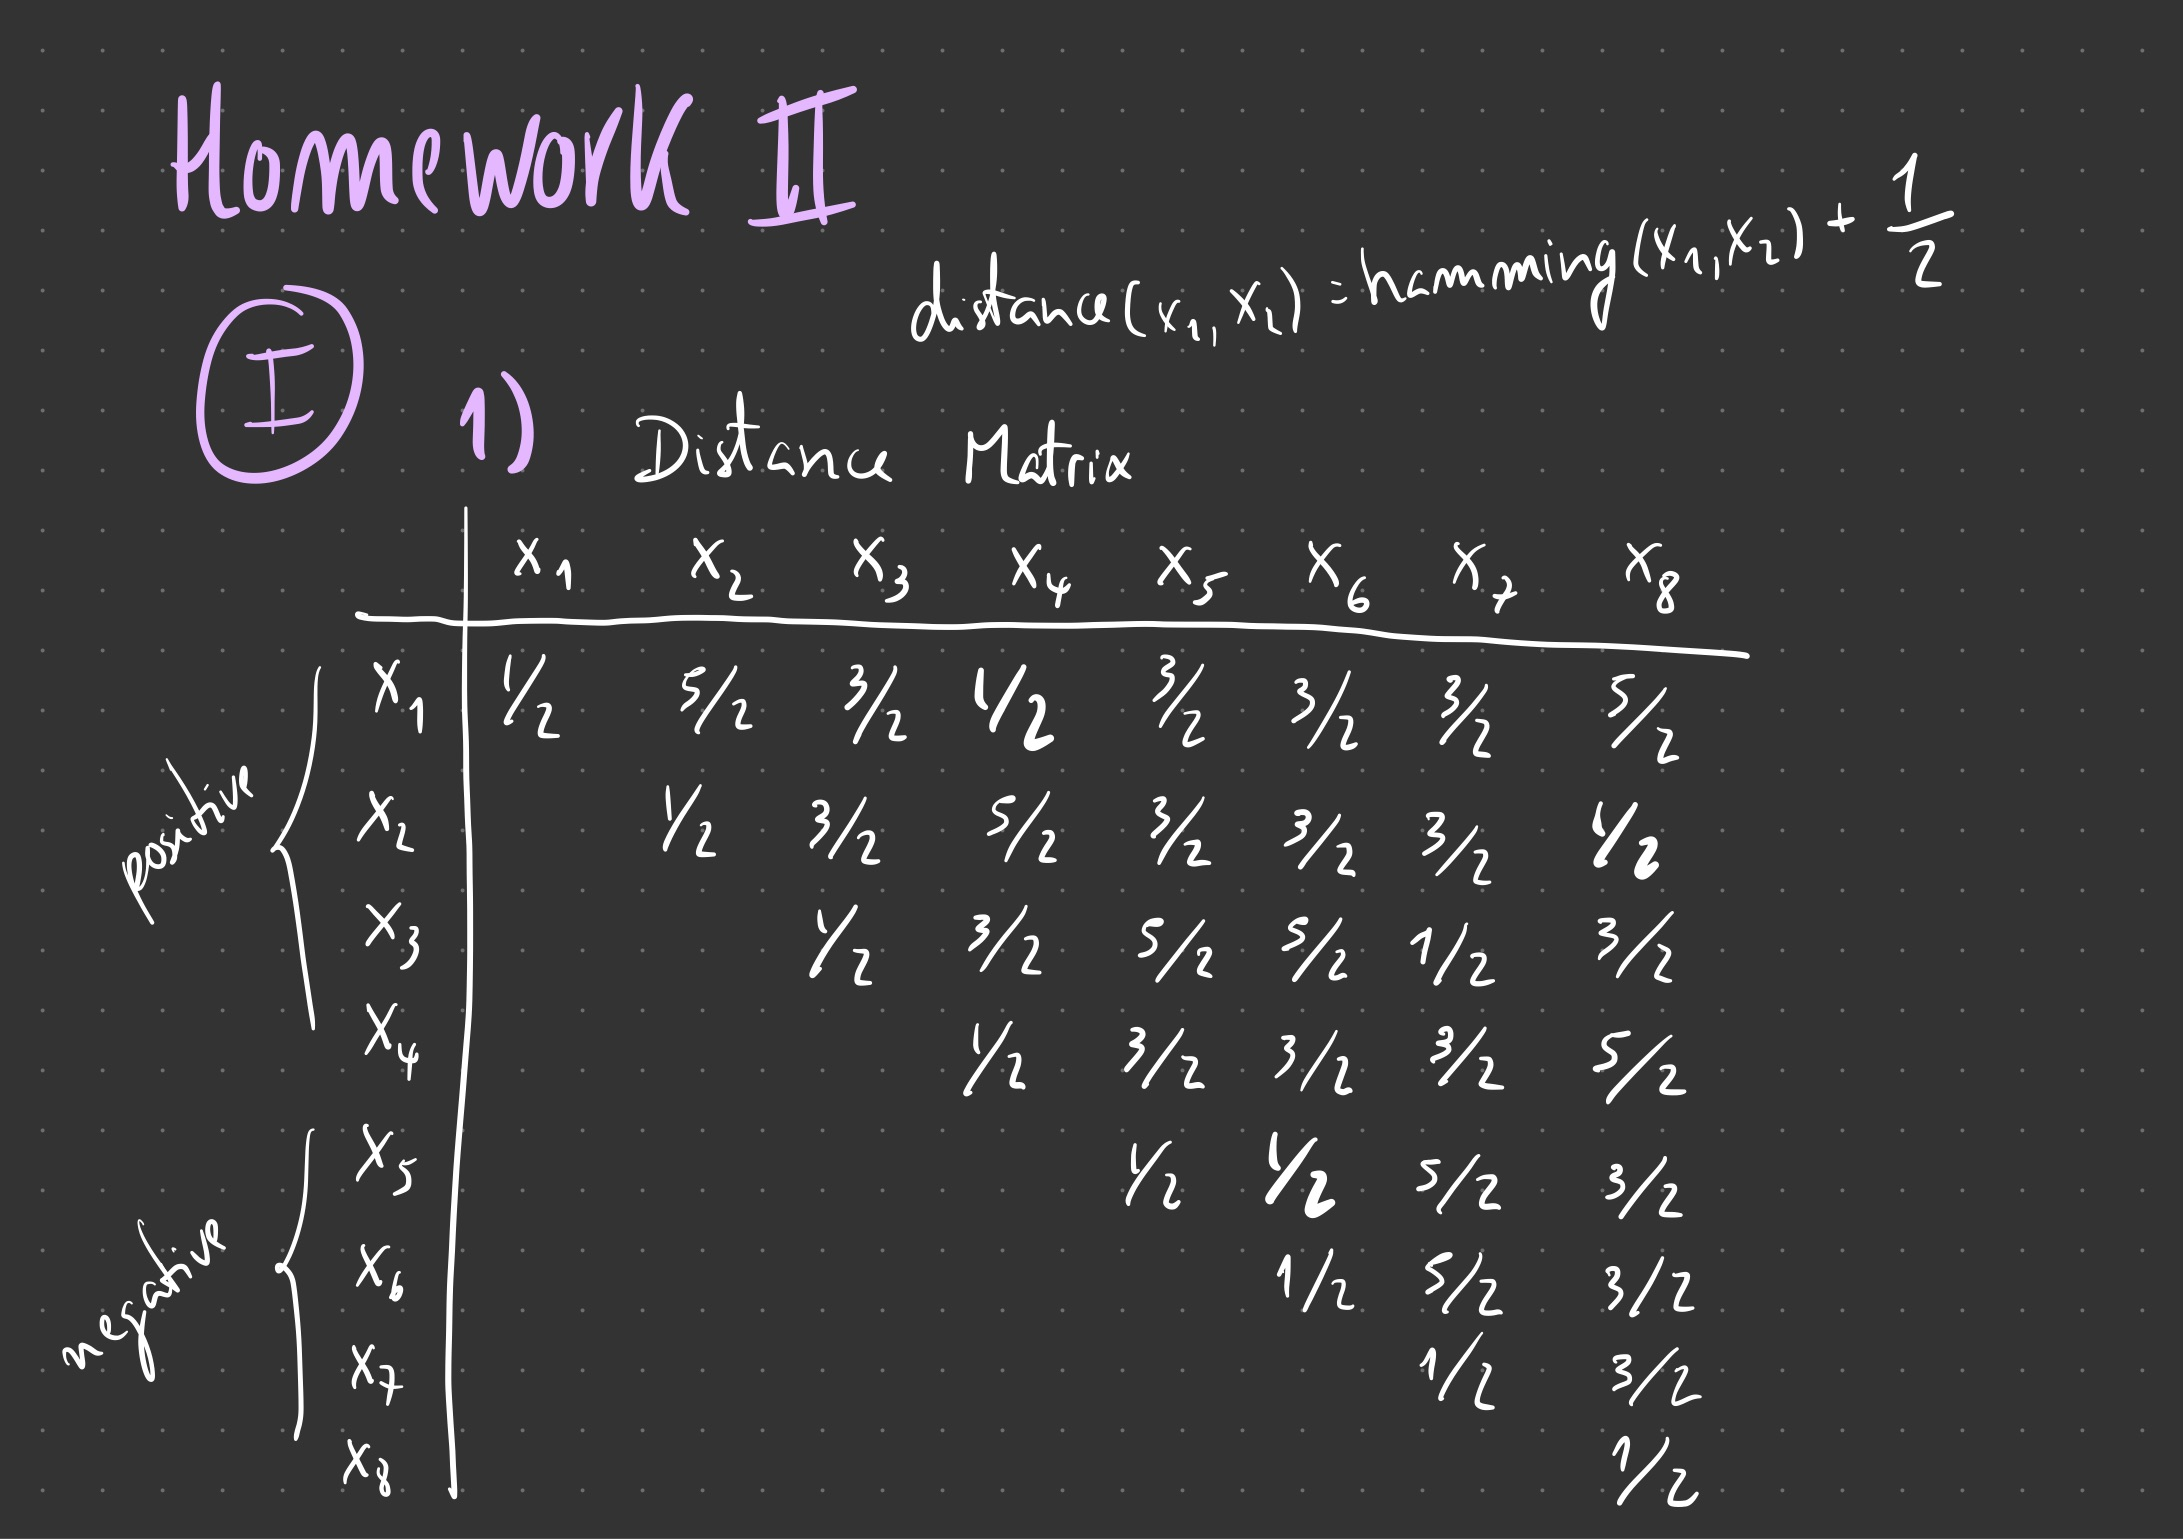
\includegraphics[scale=0.2]{images/Project-02.jpg}
\newline
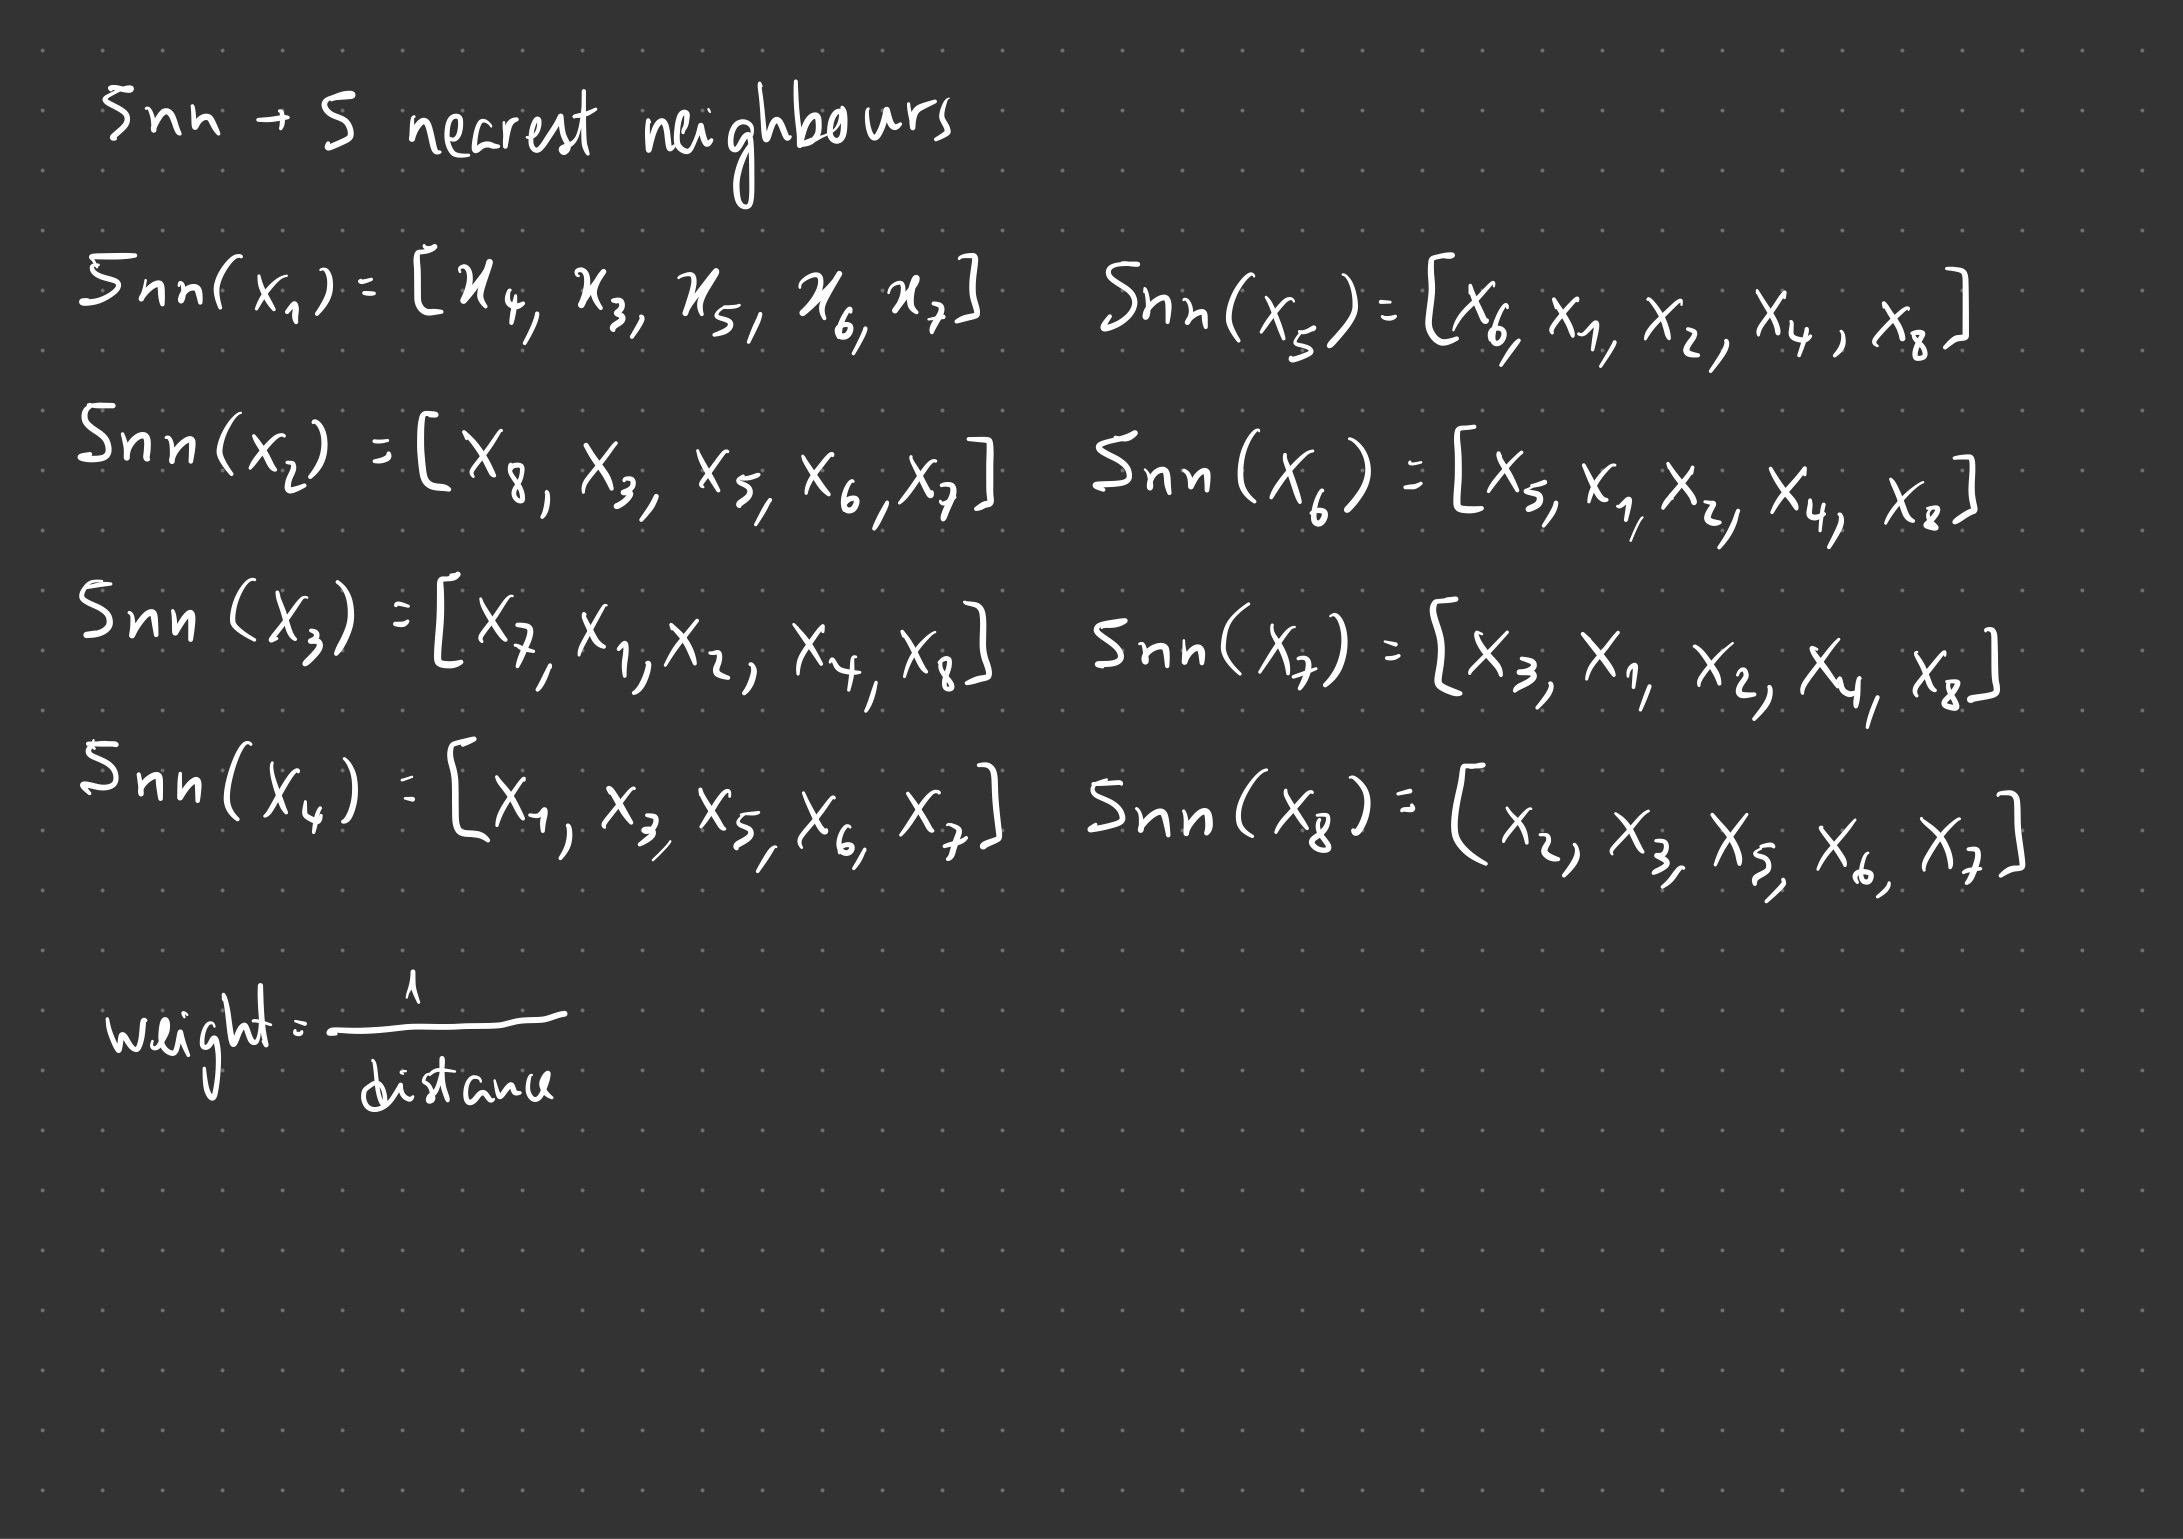
\includegraphics[scale=0.2]{images/Project-03.jpg}
\newline
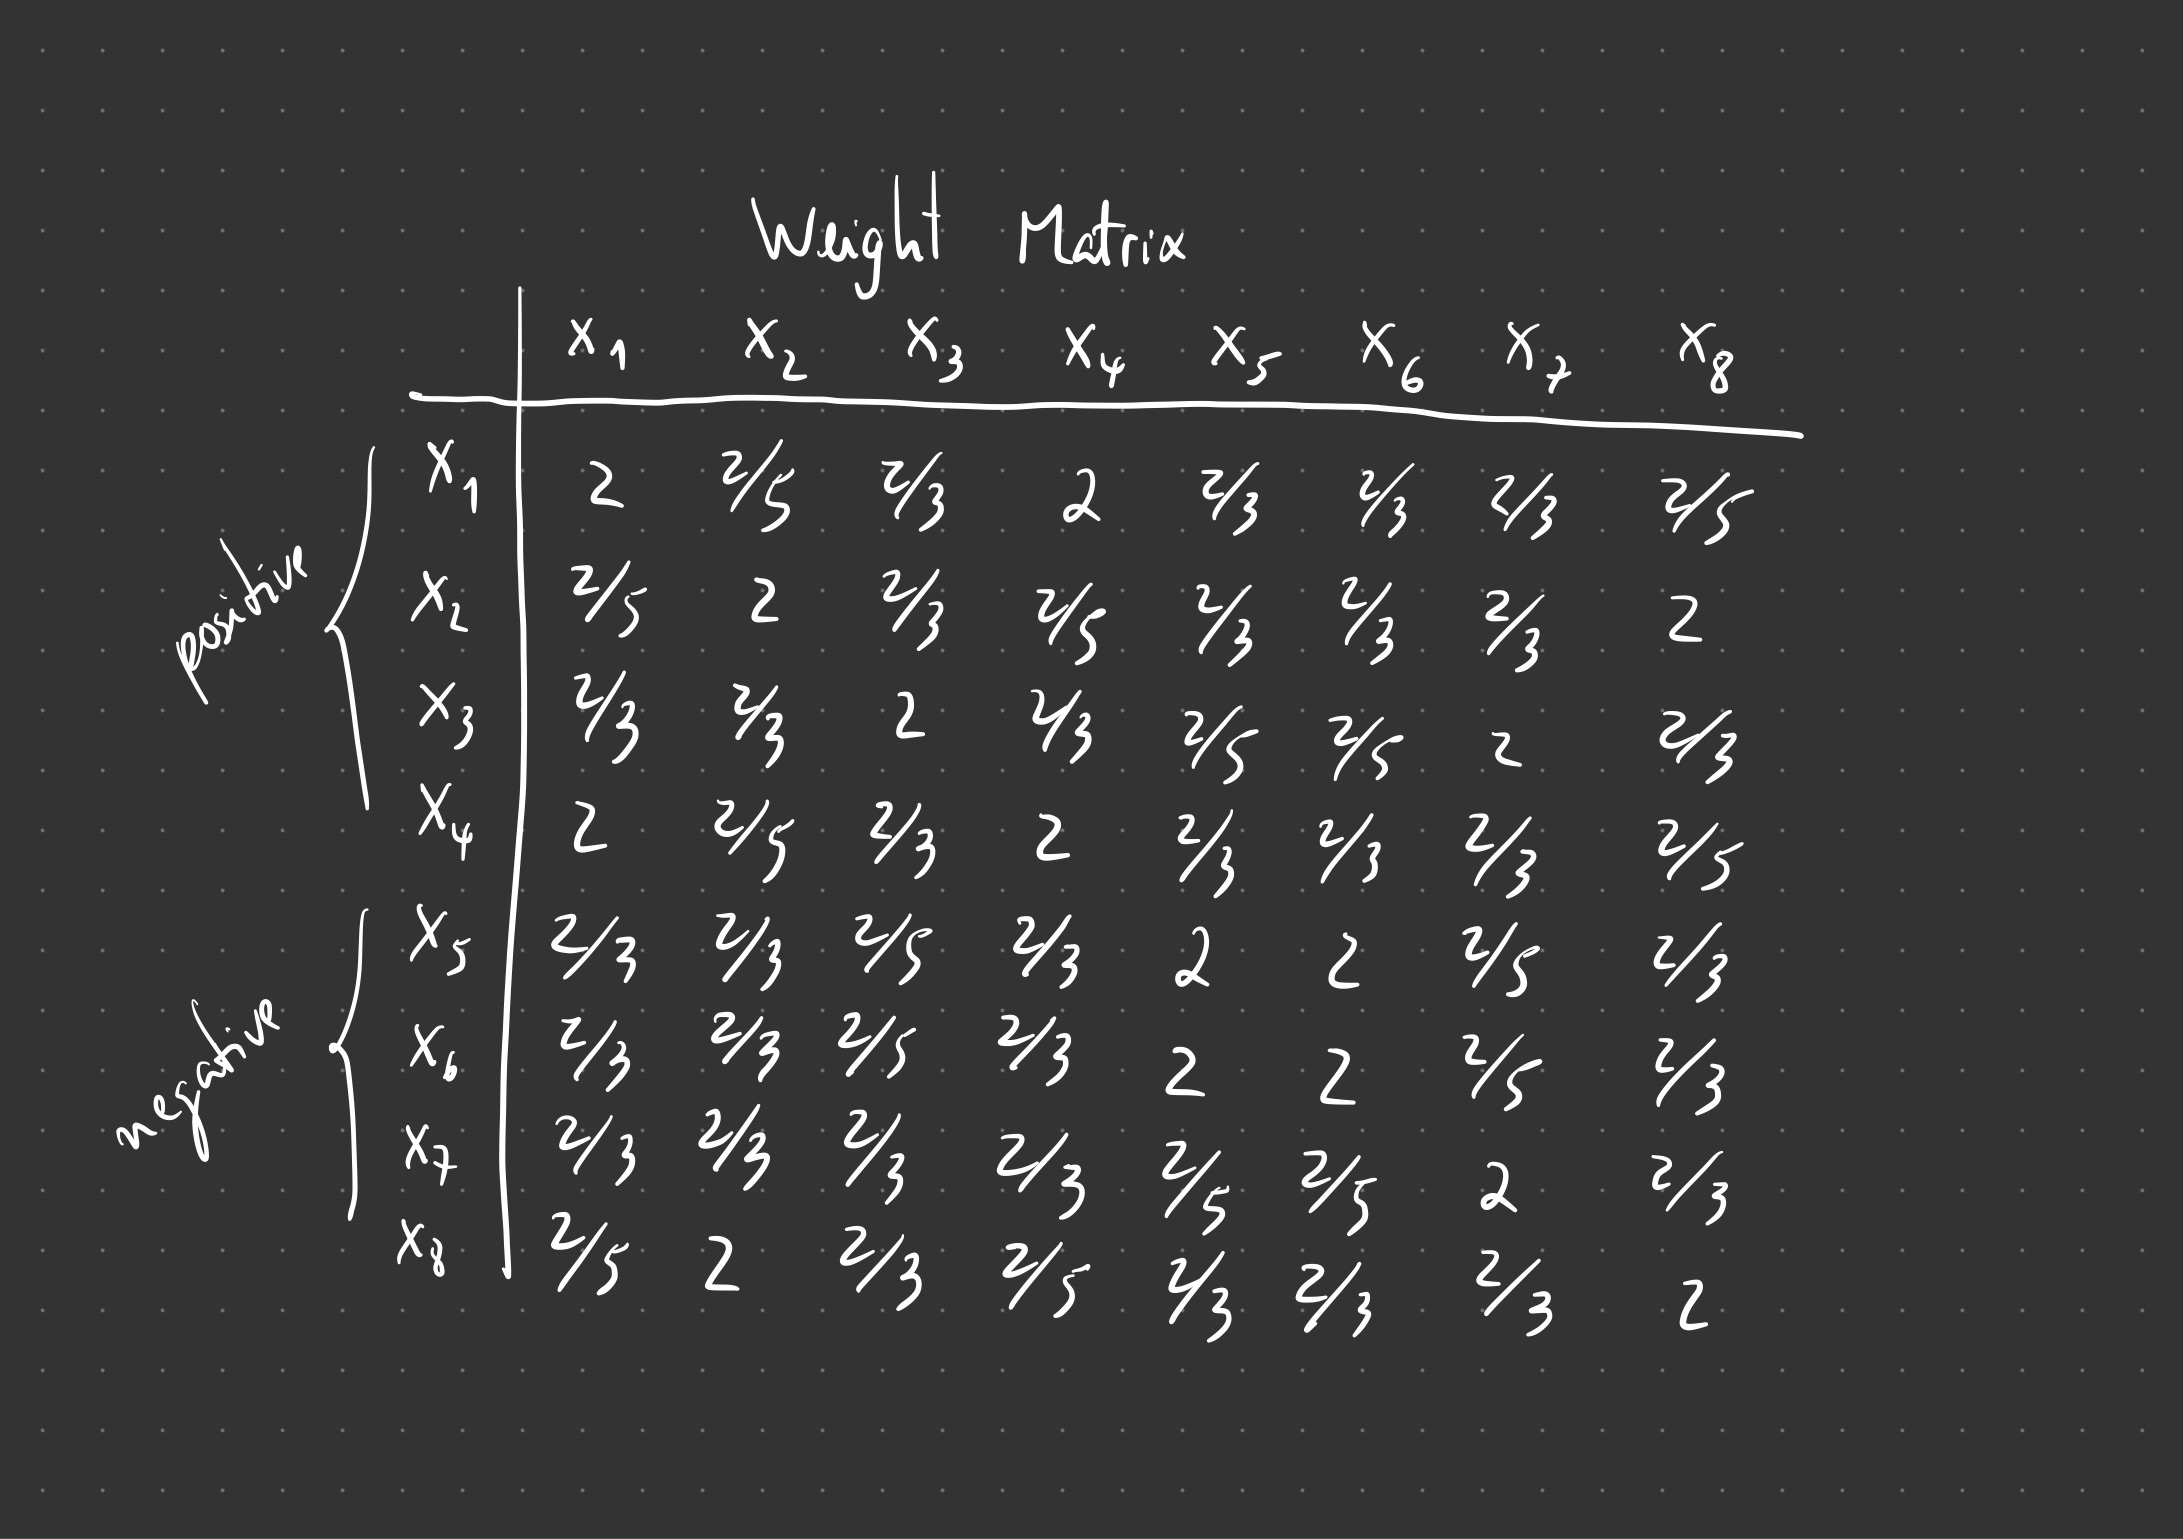
\includegraphics[scale=0.2]{images/Project-04.jpg}
\newline
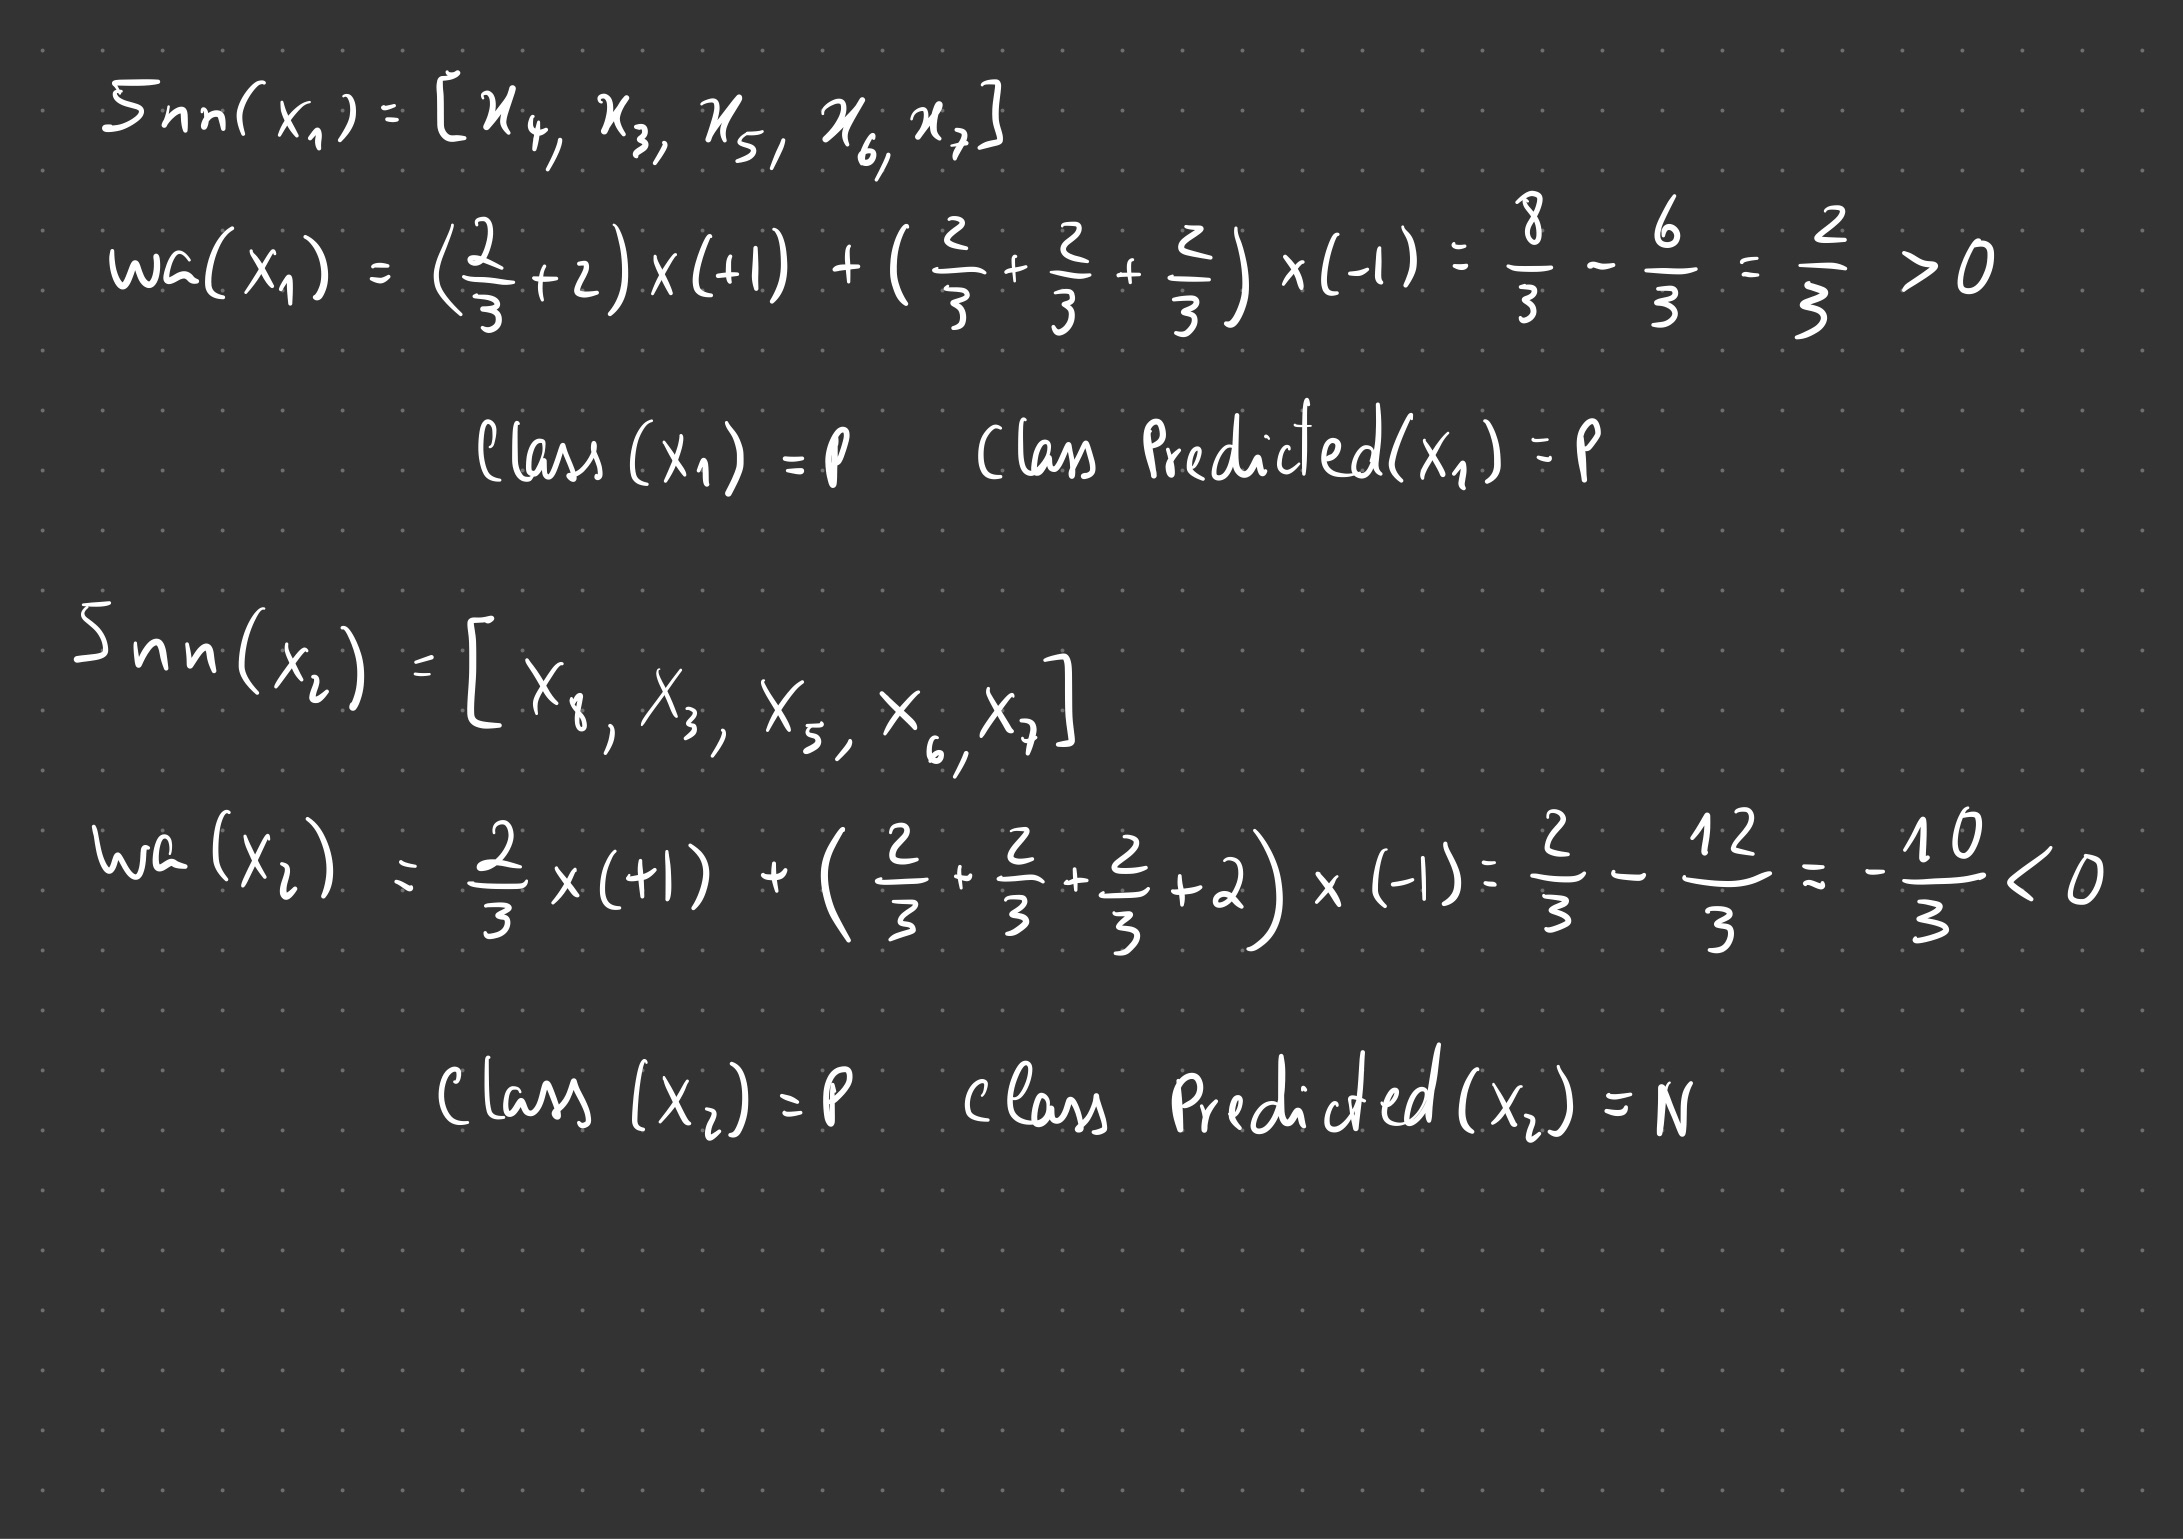
\includegraphics[scale=0.2]{images/Project-05.jpg}
\newline
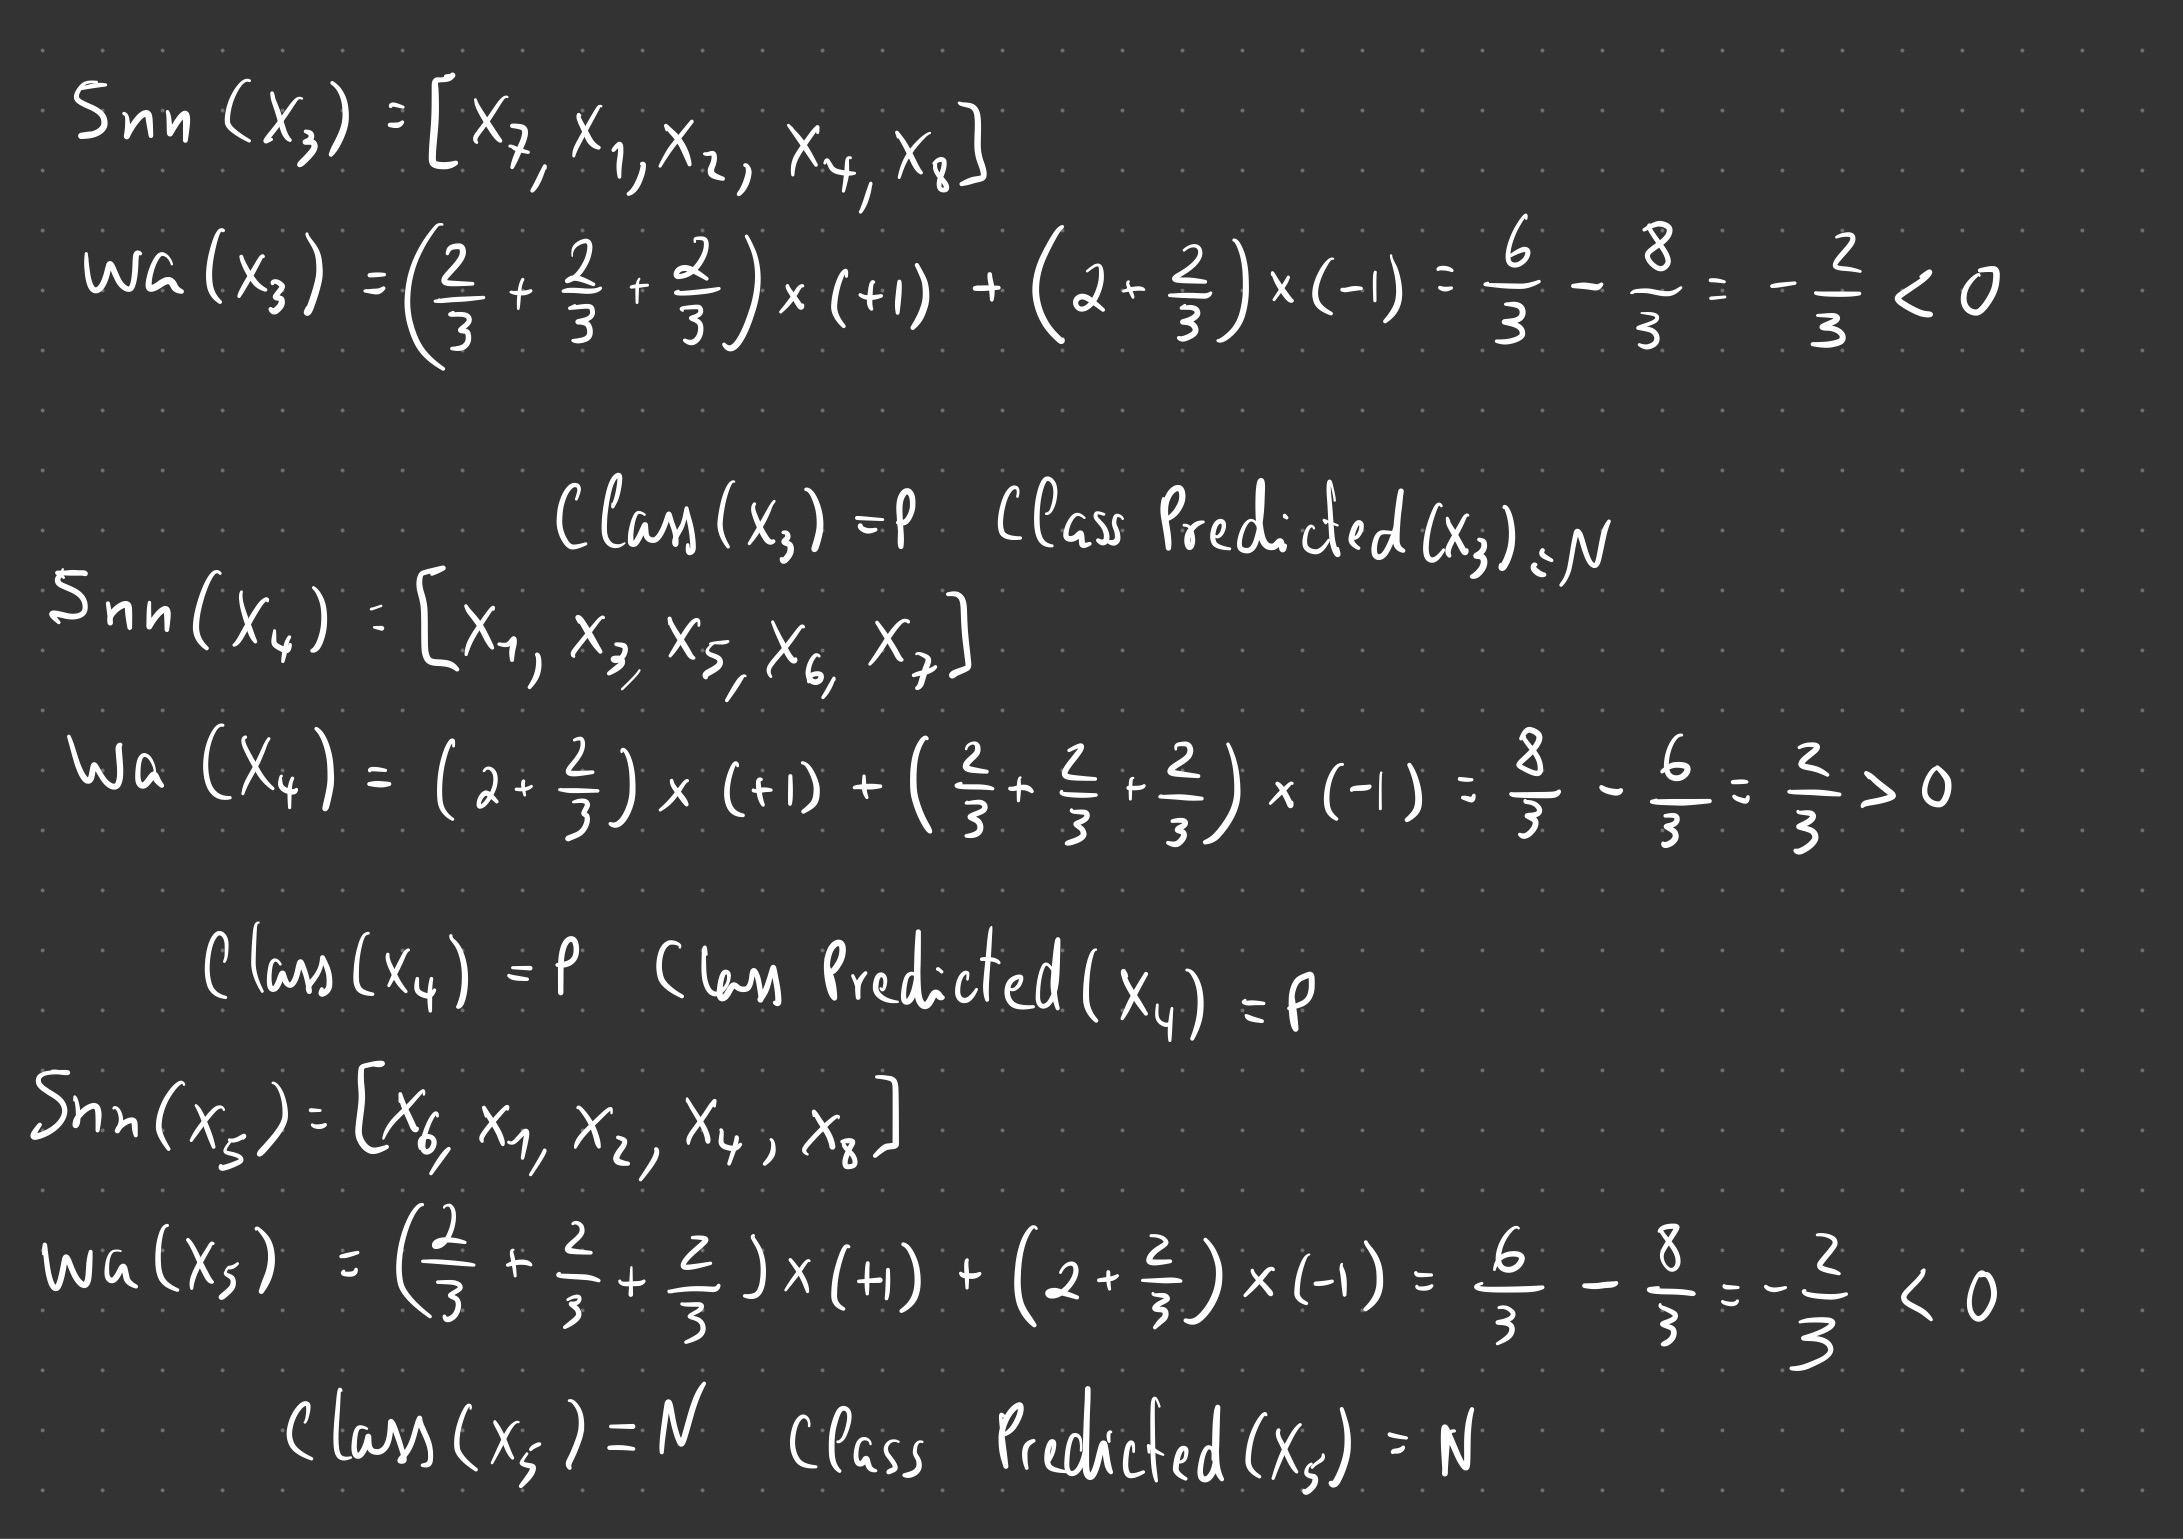
\includegraphics[scale=0.2]{images/Project-06.jpg}
\newline
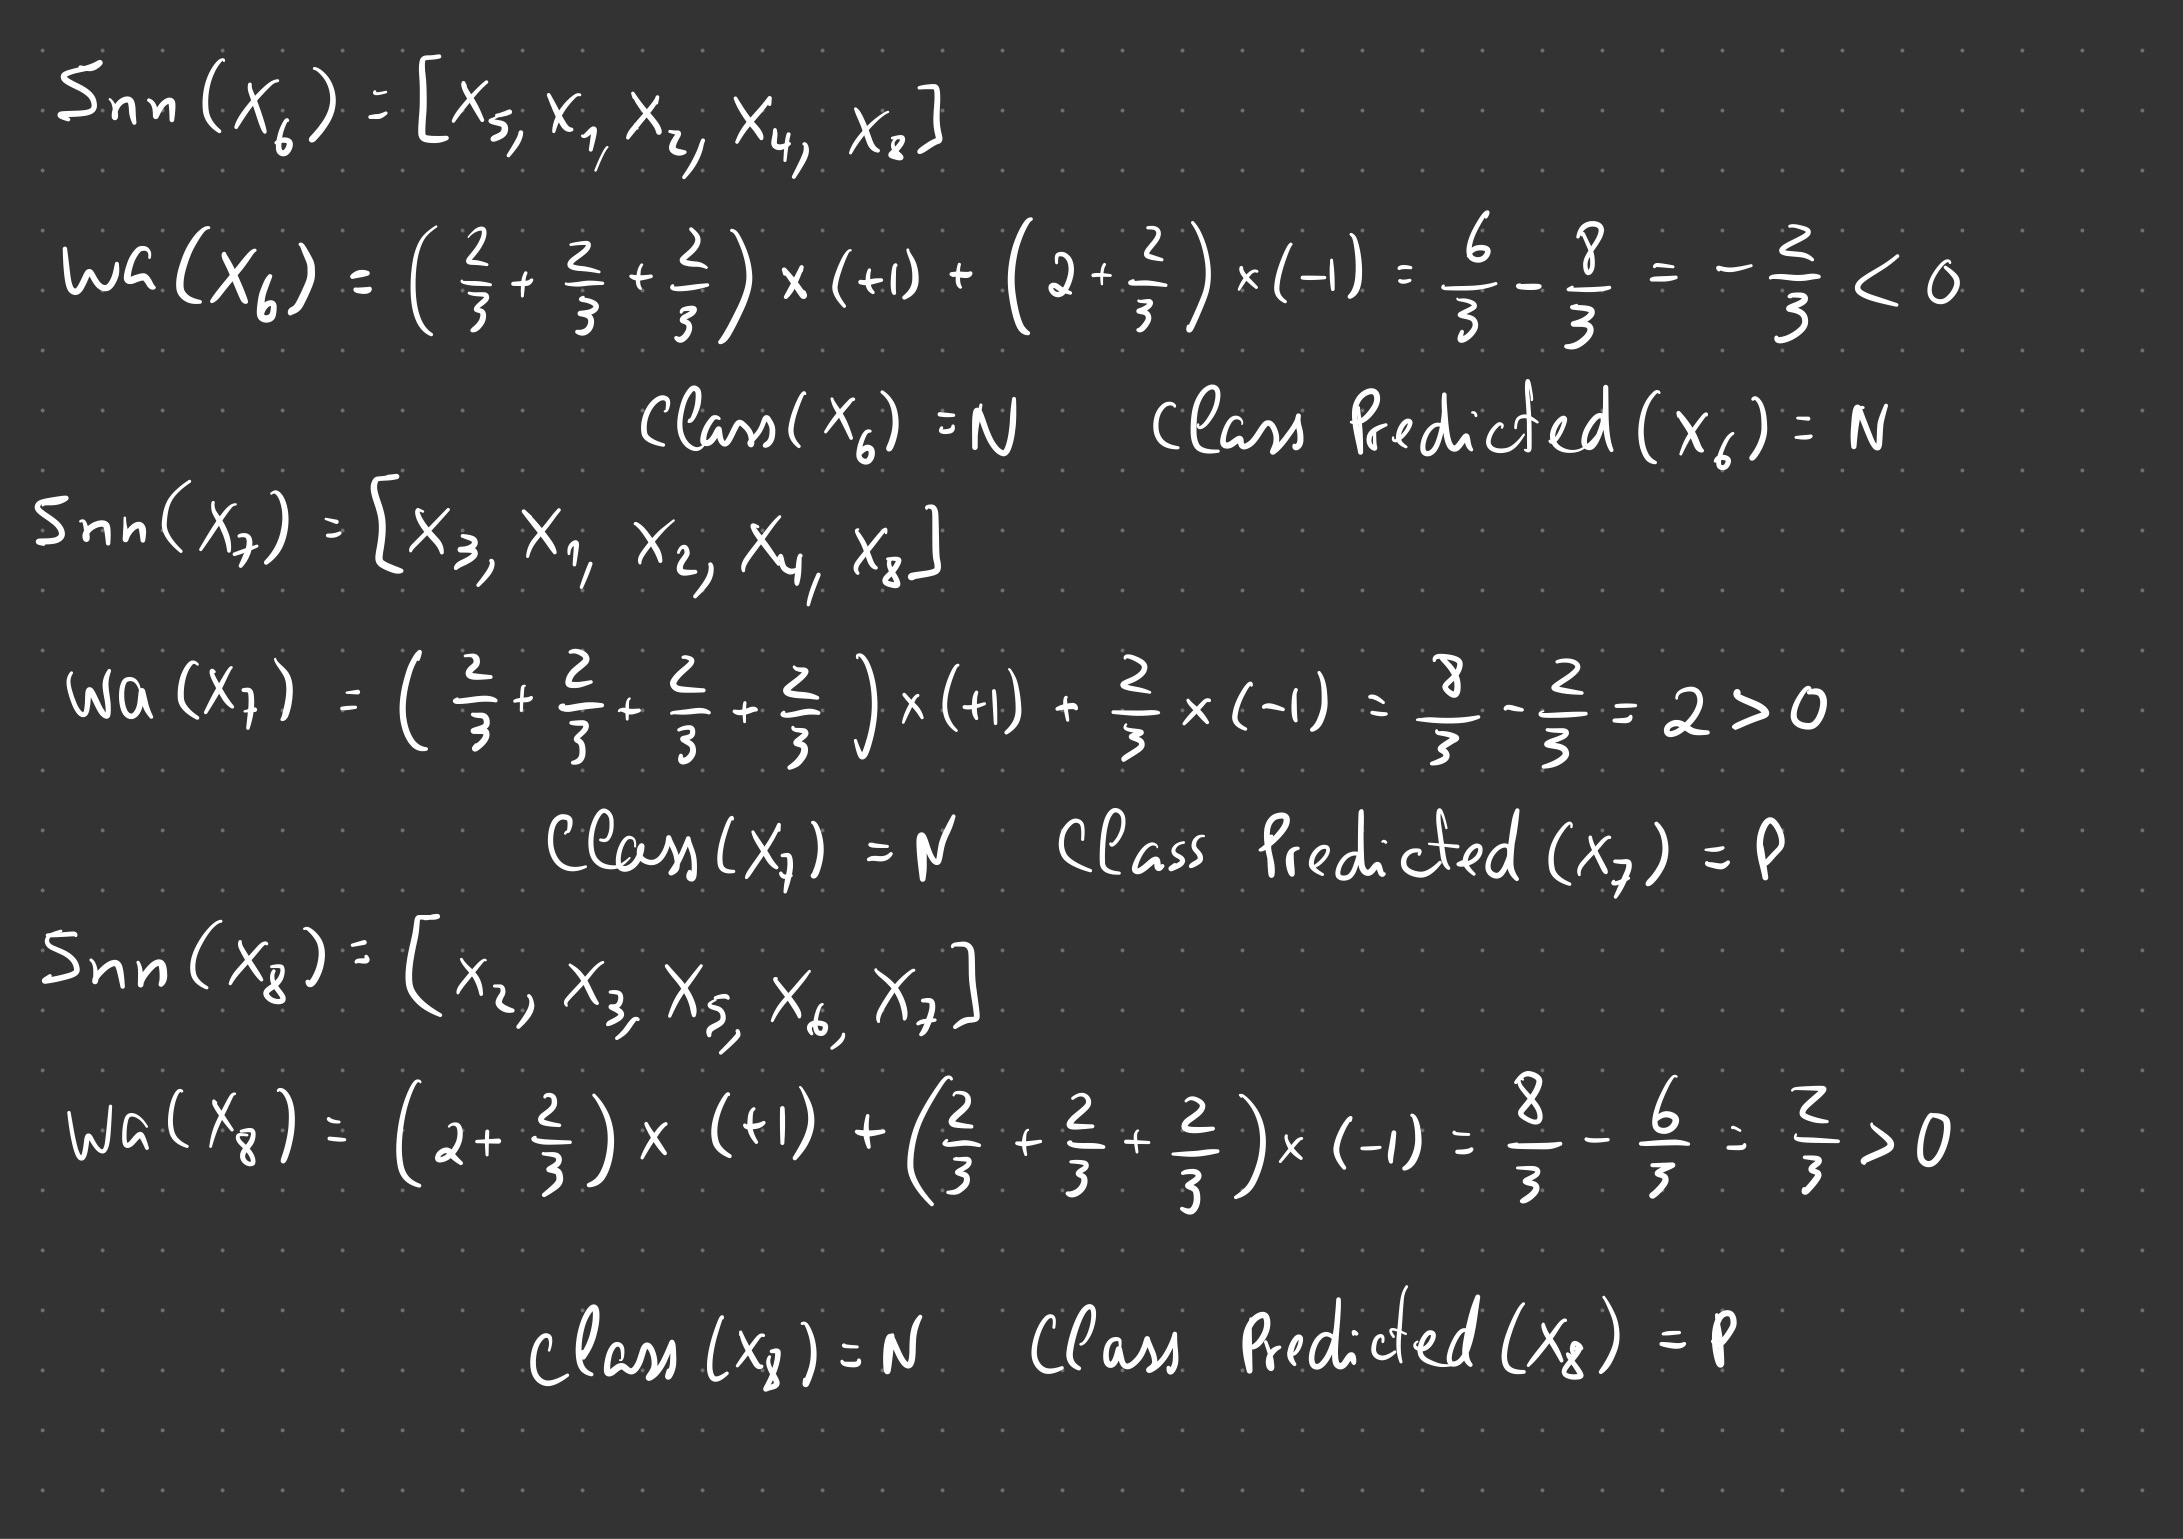
\includegraphics[scale=0.2]{images/Project-07.jpg}
\newline
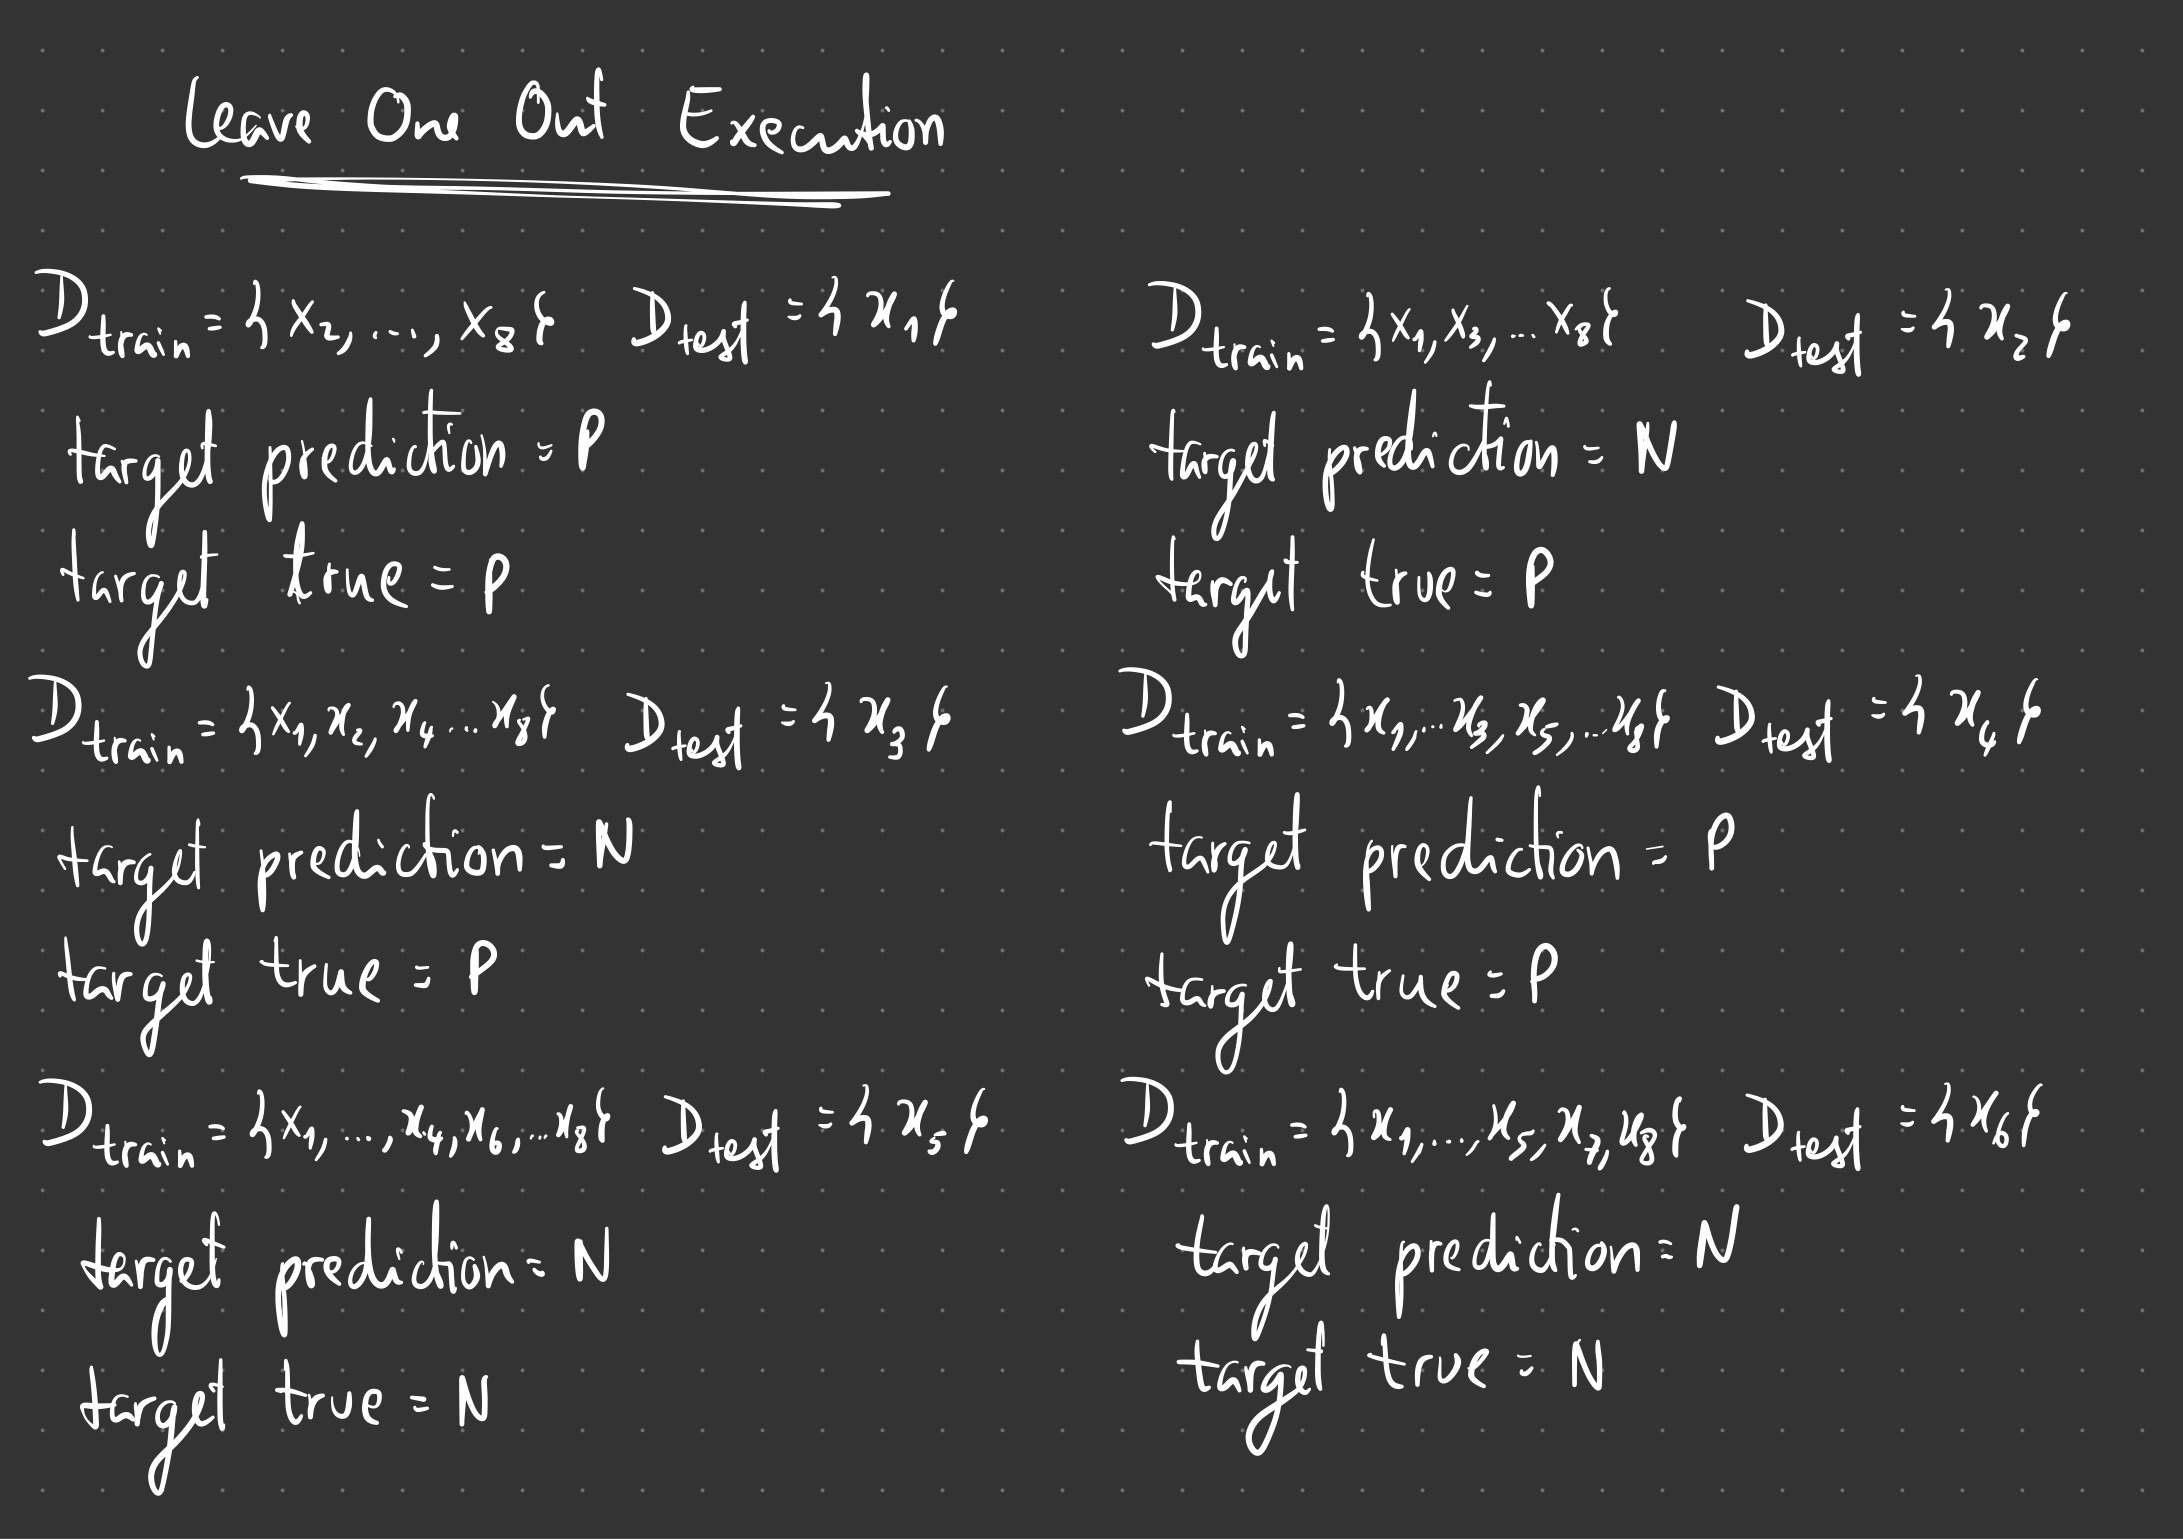
\includegraphics[scale=0.2]{images/Project-08.jpg}
\newline
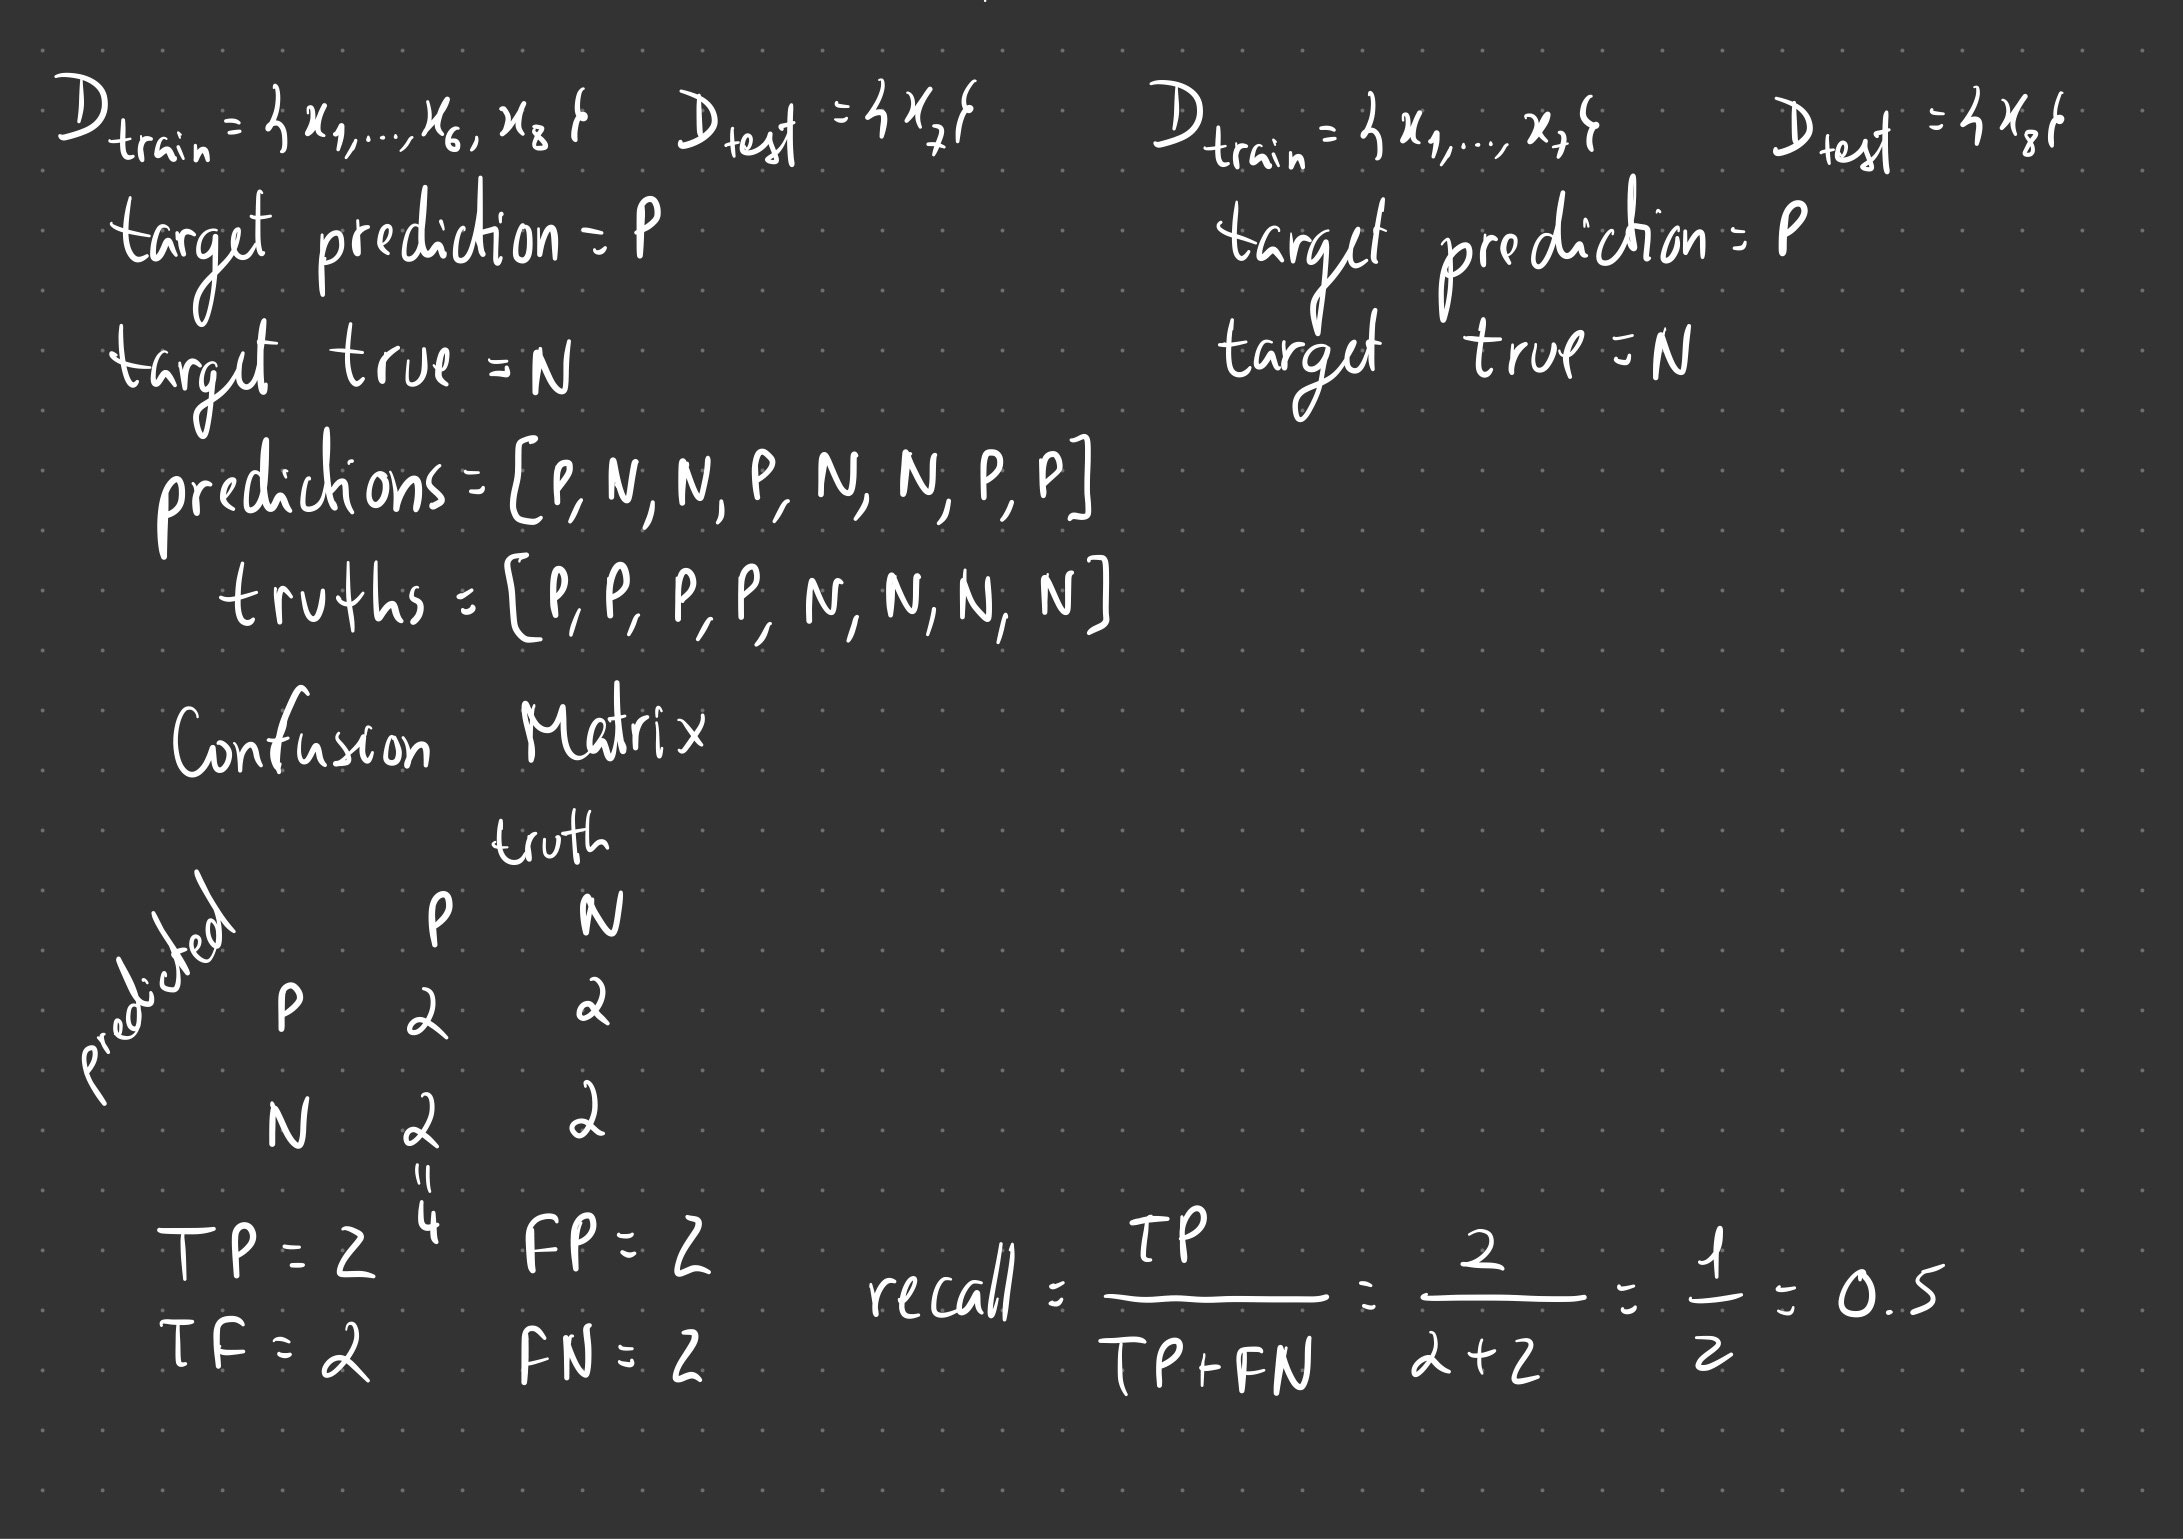
\includegraphics[scale=0.2]{images/Project-09.jpg}
\newline
\end{center}
\newpage

\item \leavevmode\vadjust{\vspace{-\baselineskip}}
\begin{center}
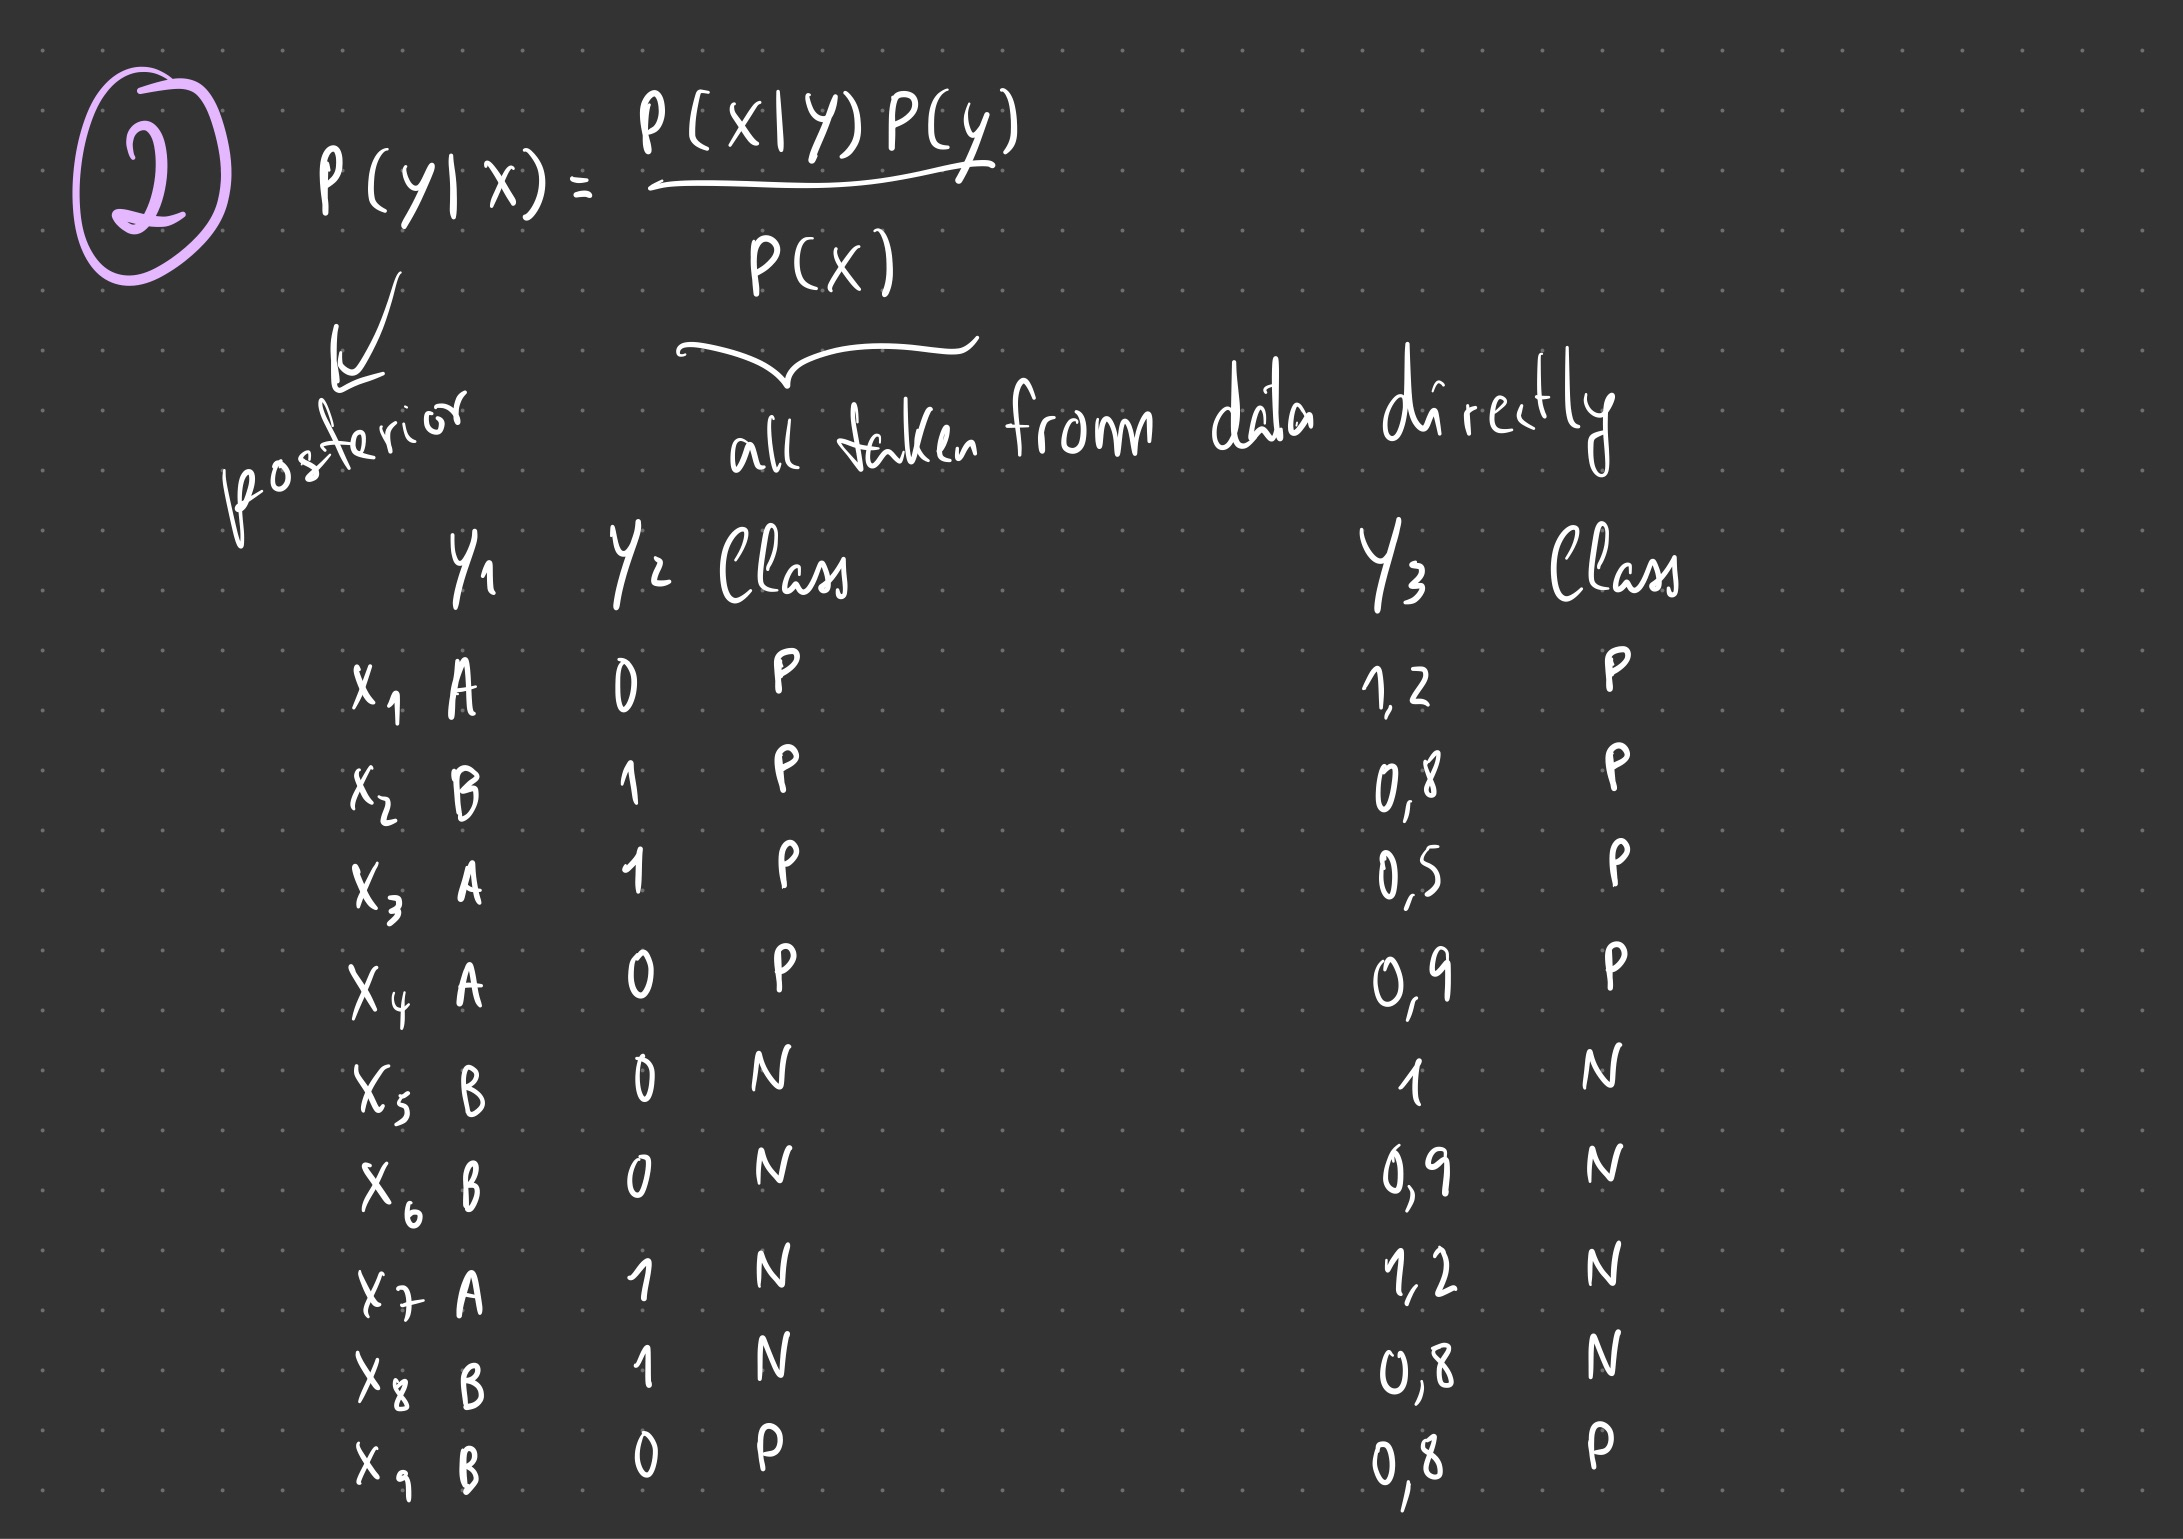
\includegraphics[scale=0.2]{images/Project-10.jpg}
\newline
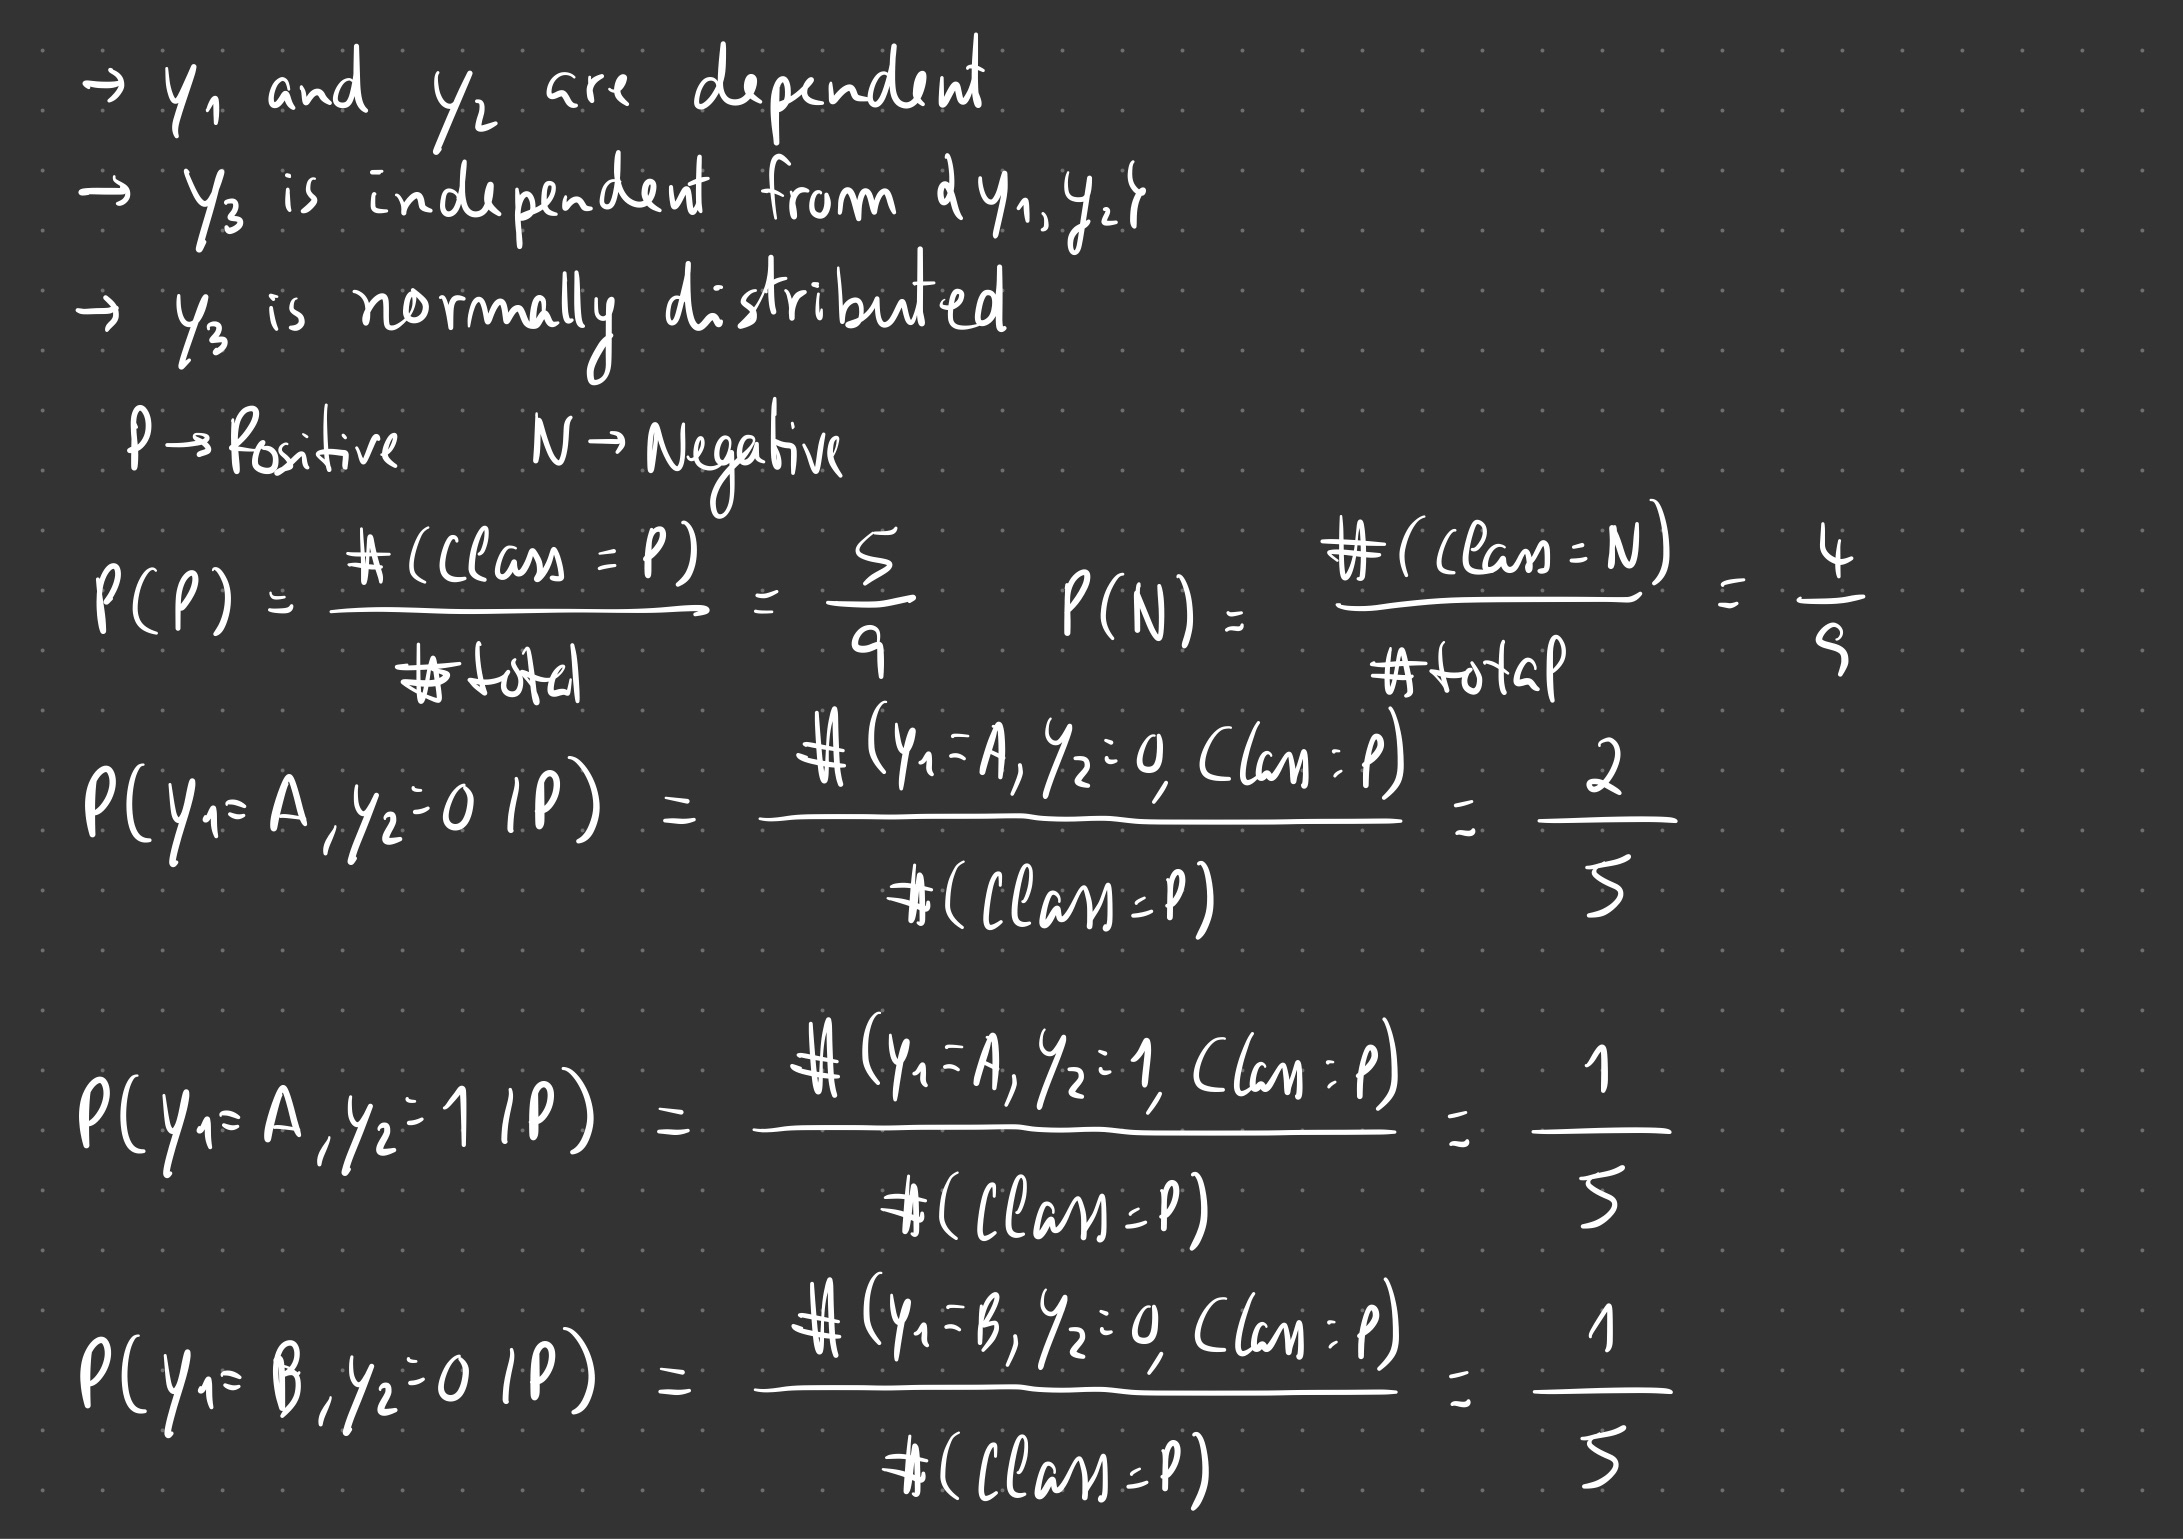
\includegraphics[scale=0.2]{images/Project-12.jpg}
\newline
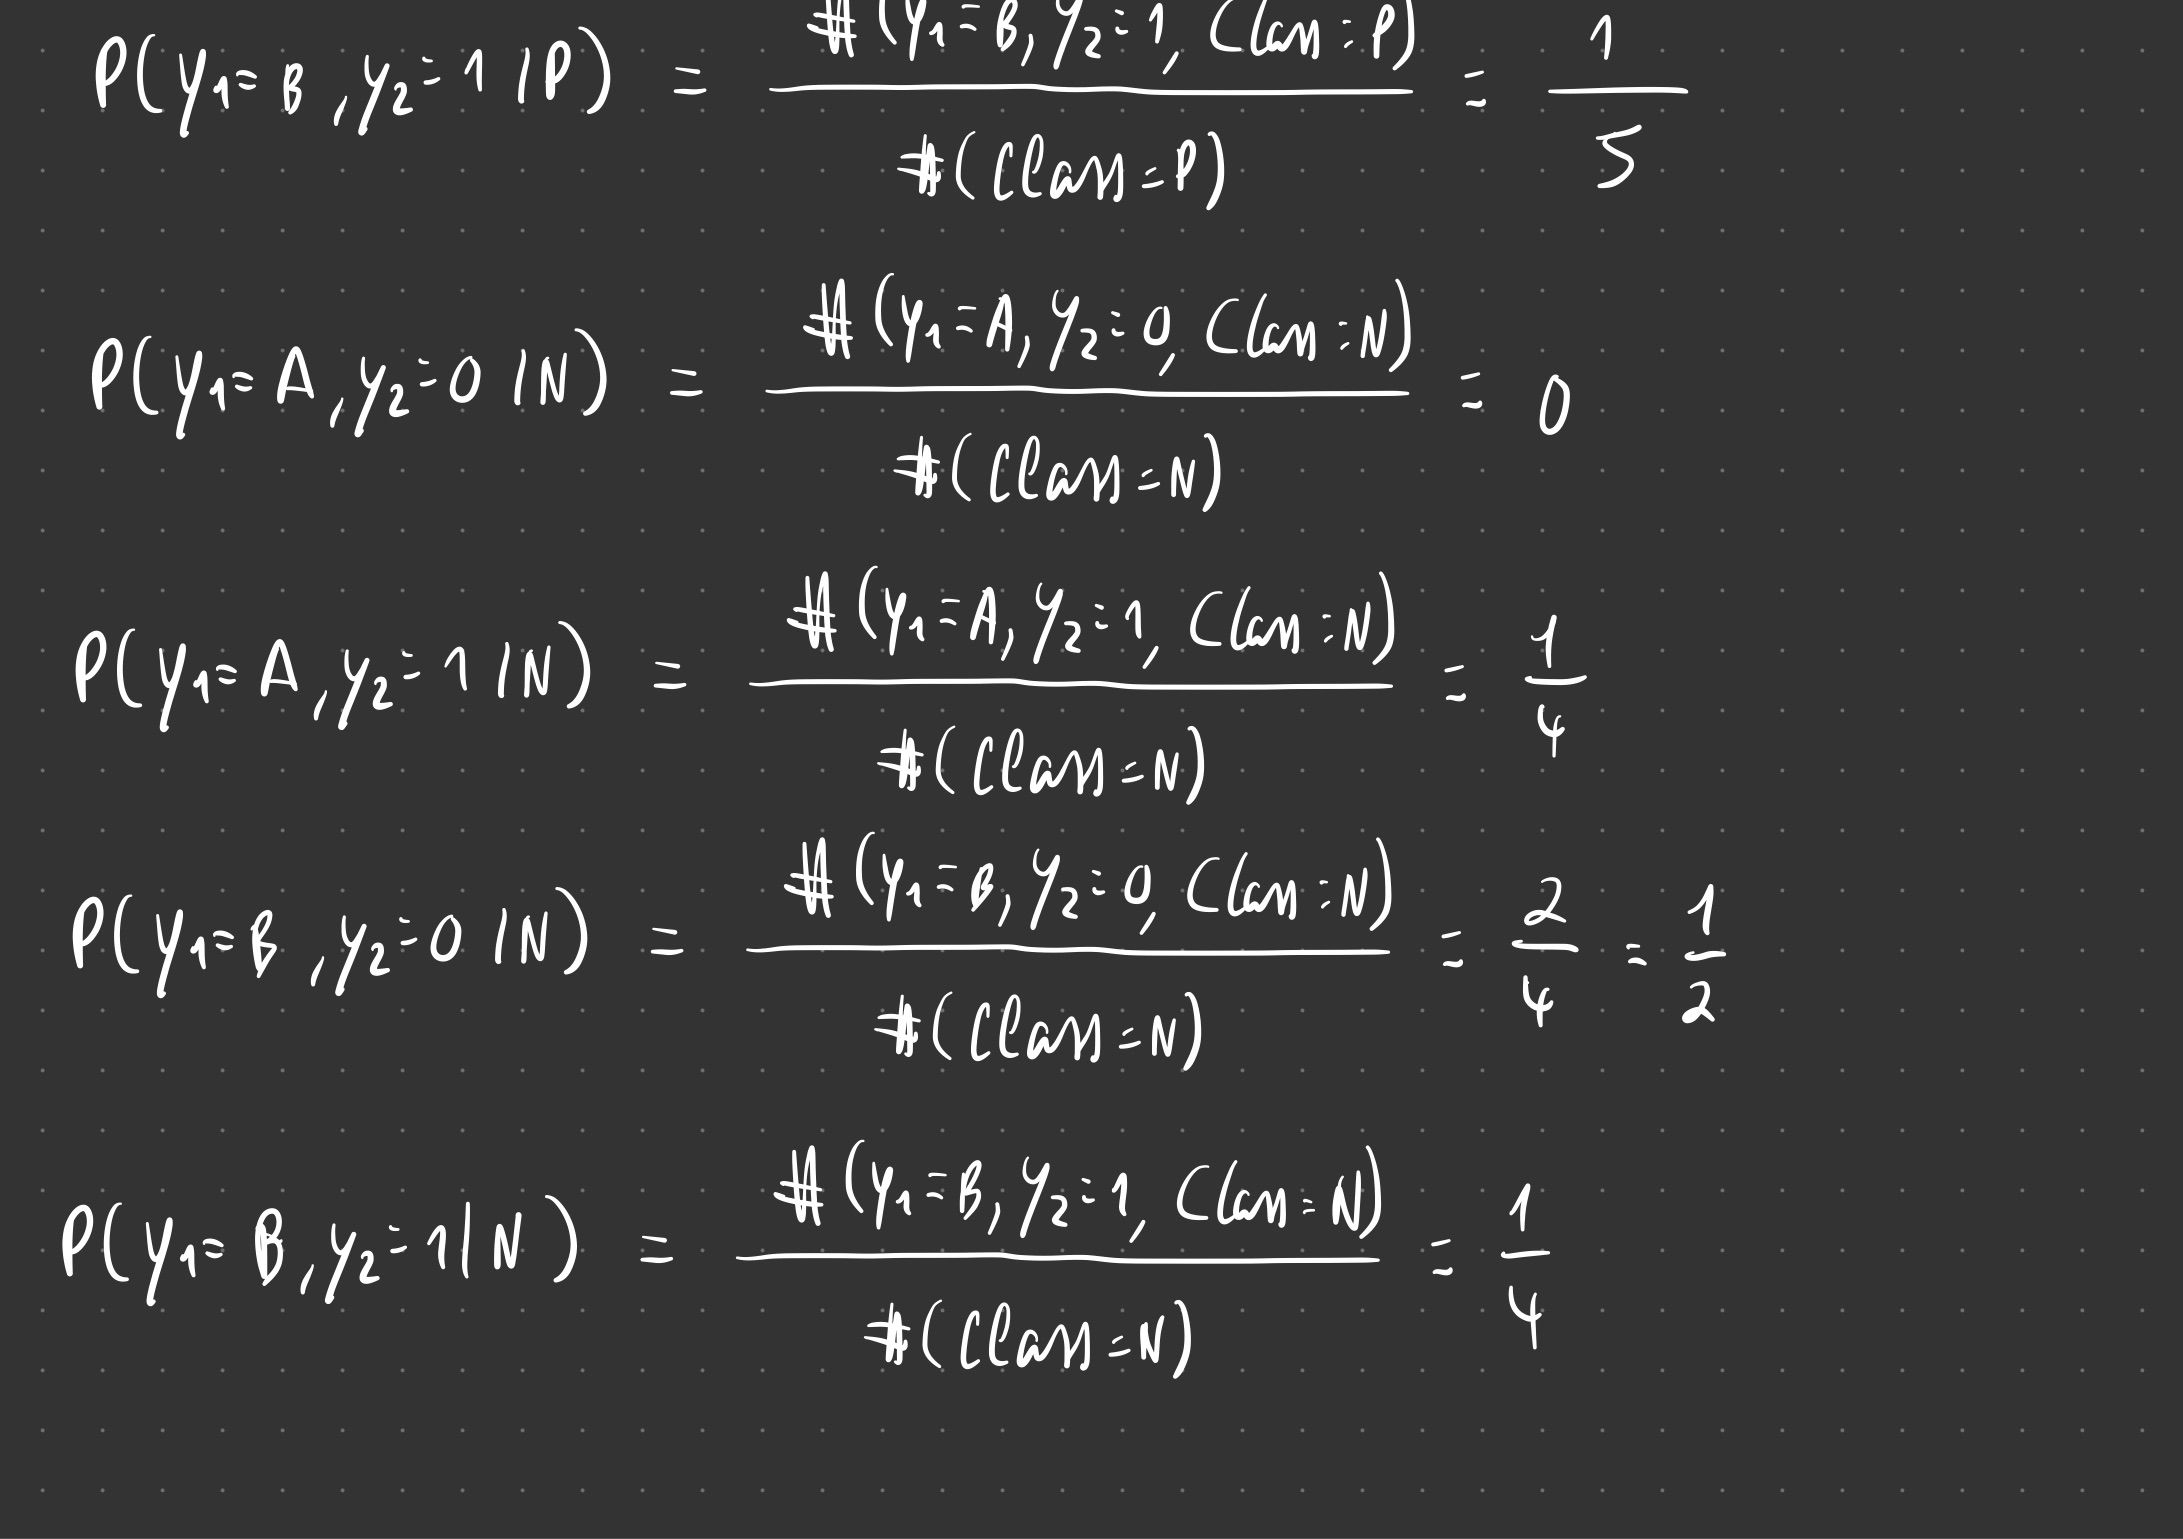
\includegraphics[scale=0.2]{images/Project-13.jpg}
\newline
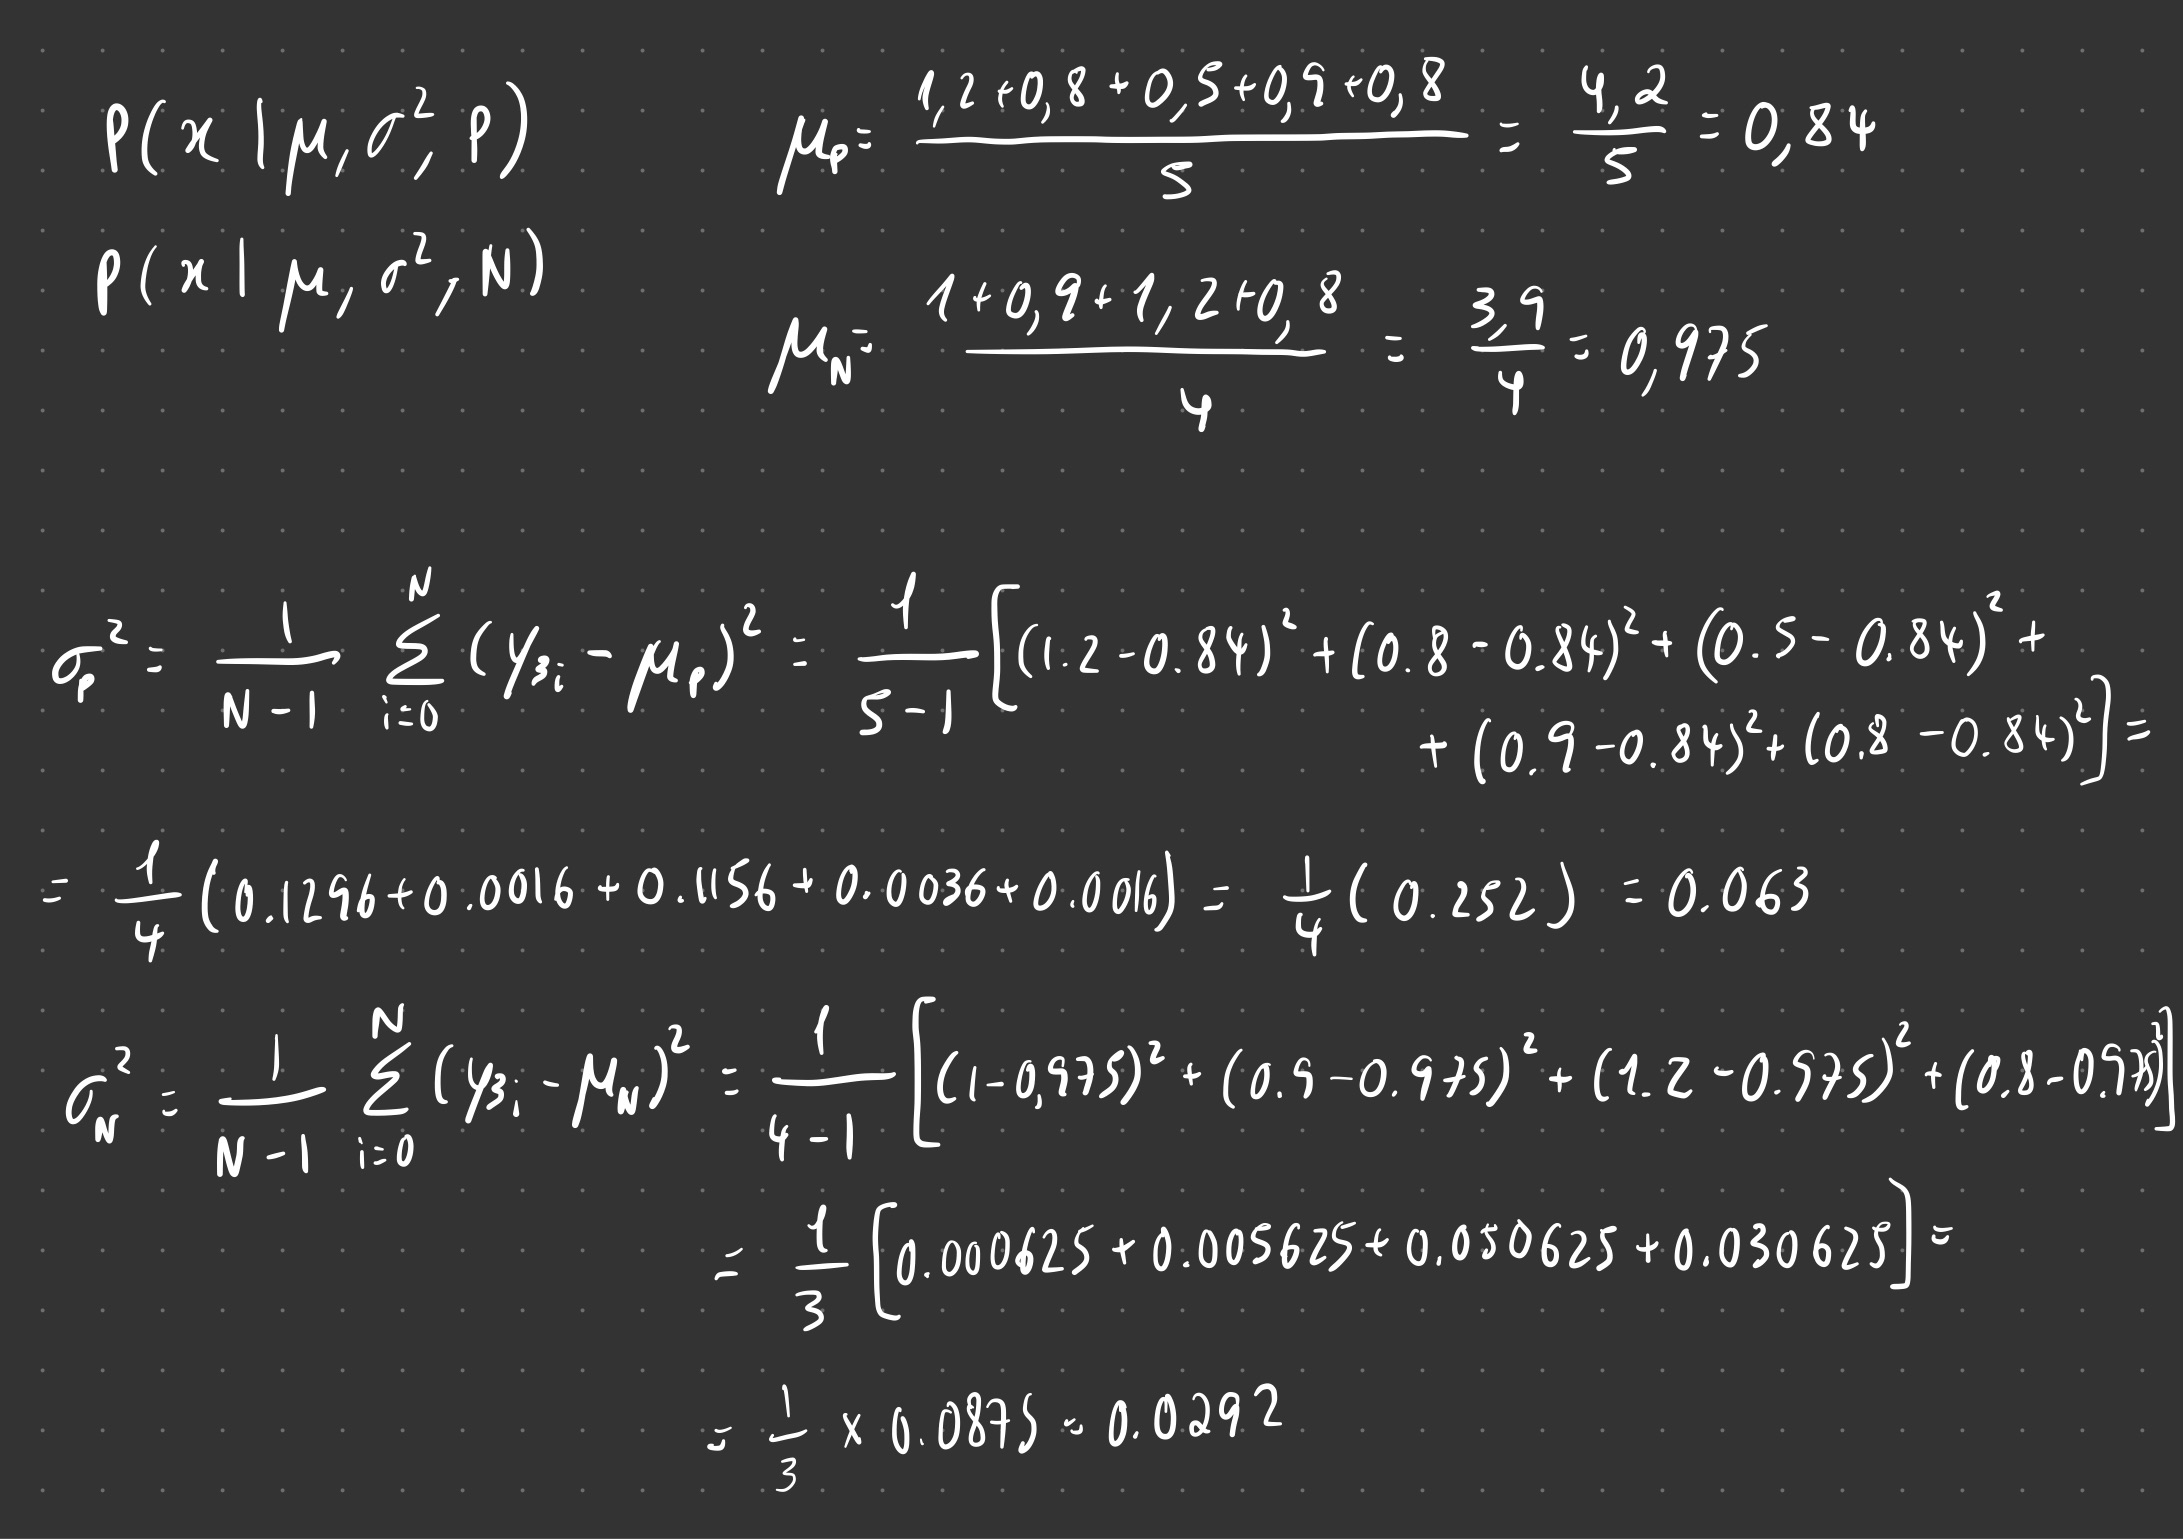
\includegraphics[scale=0.2]{images/Project-14.jpg}
\newline
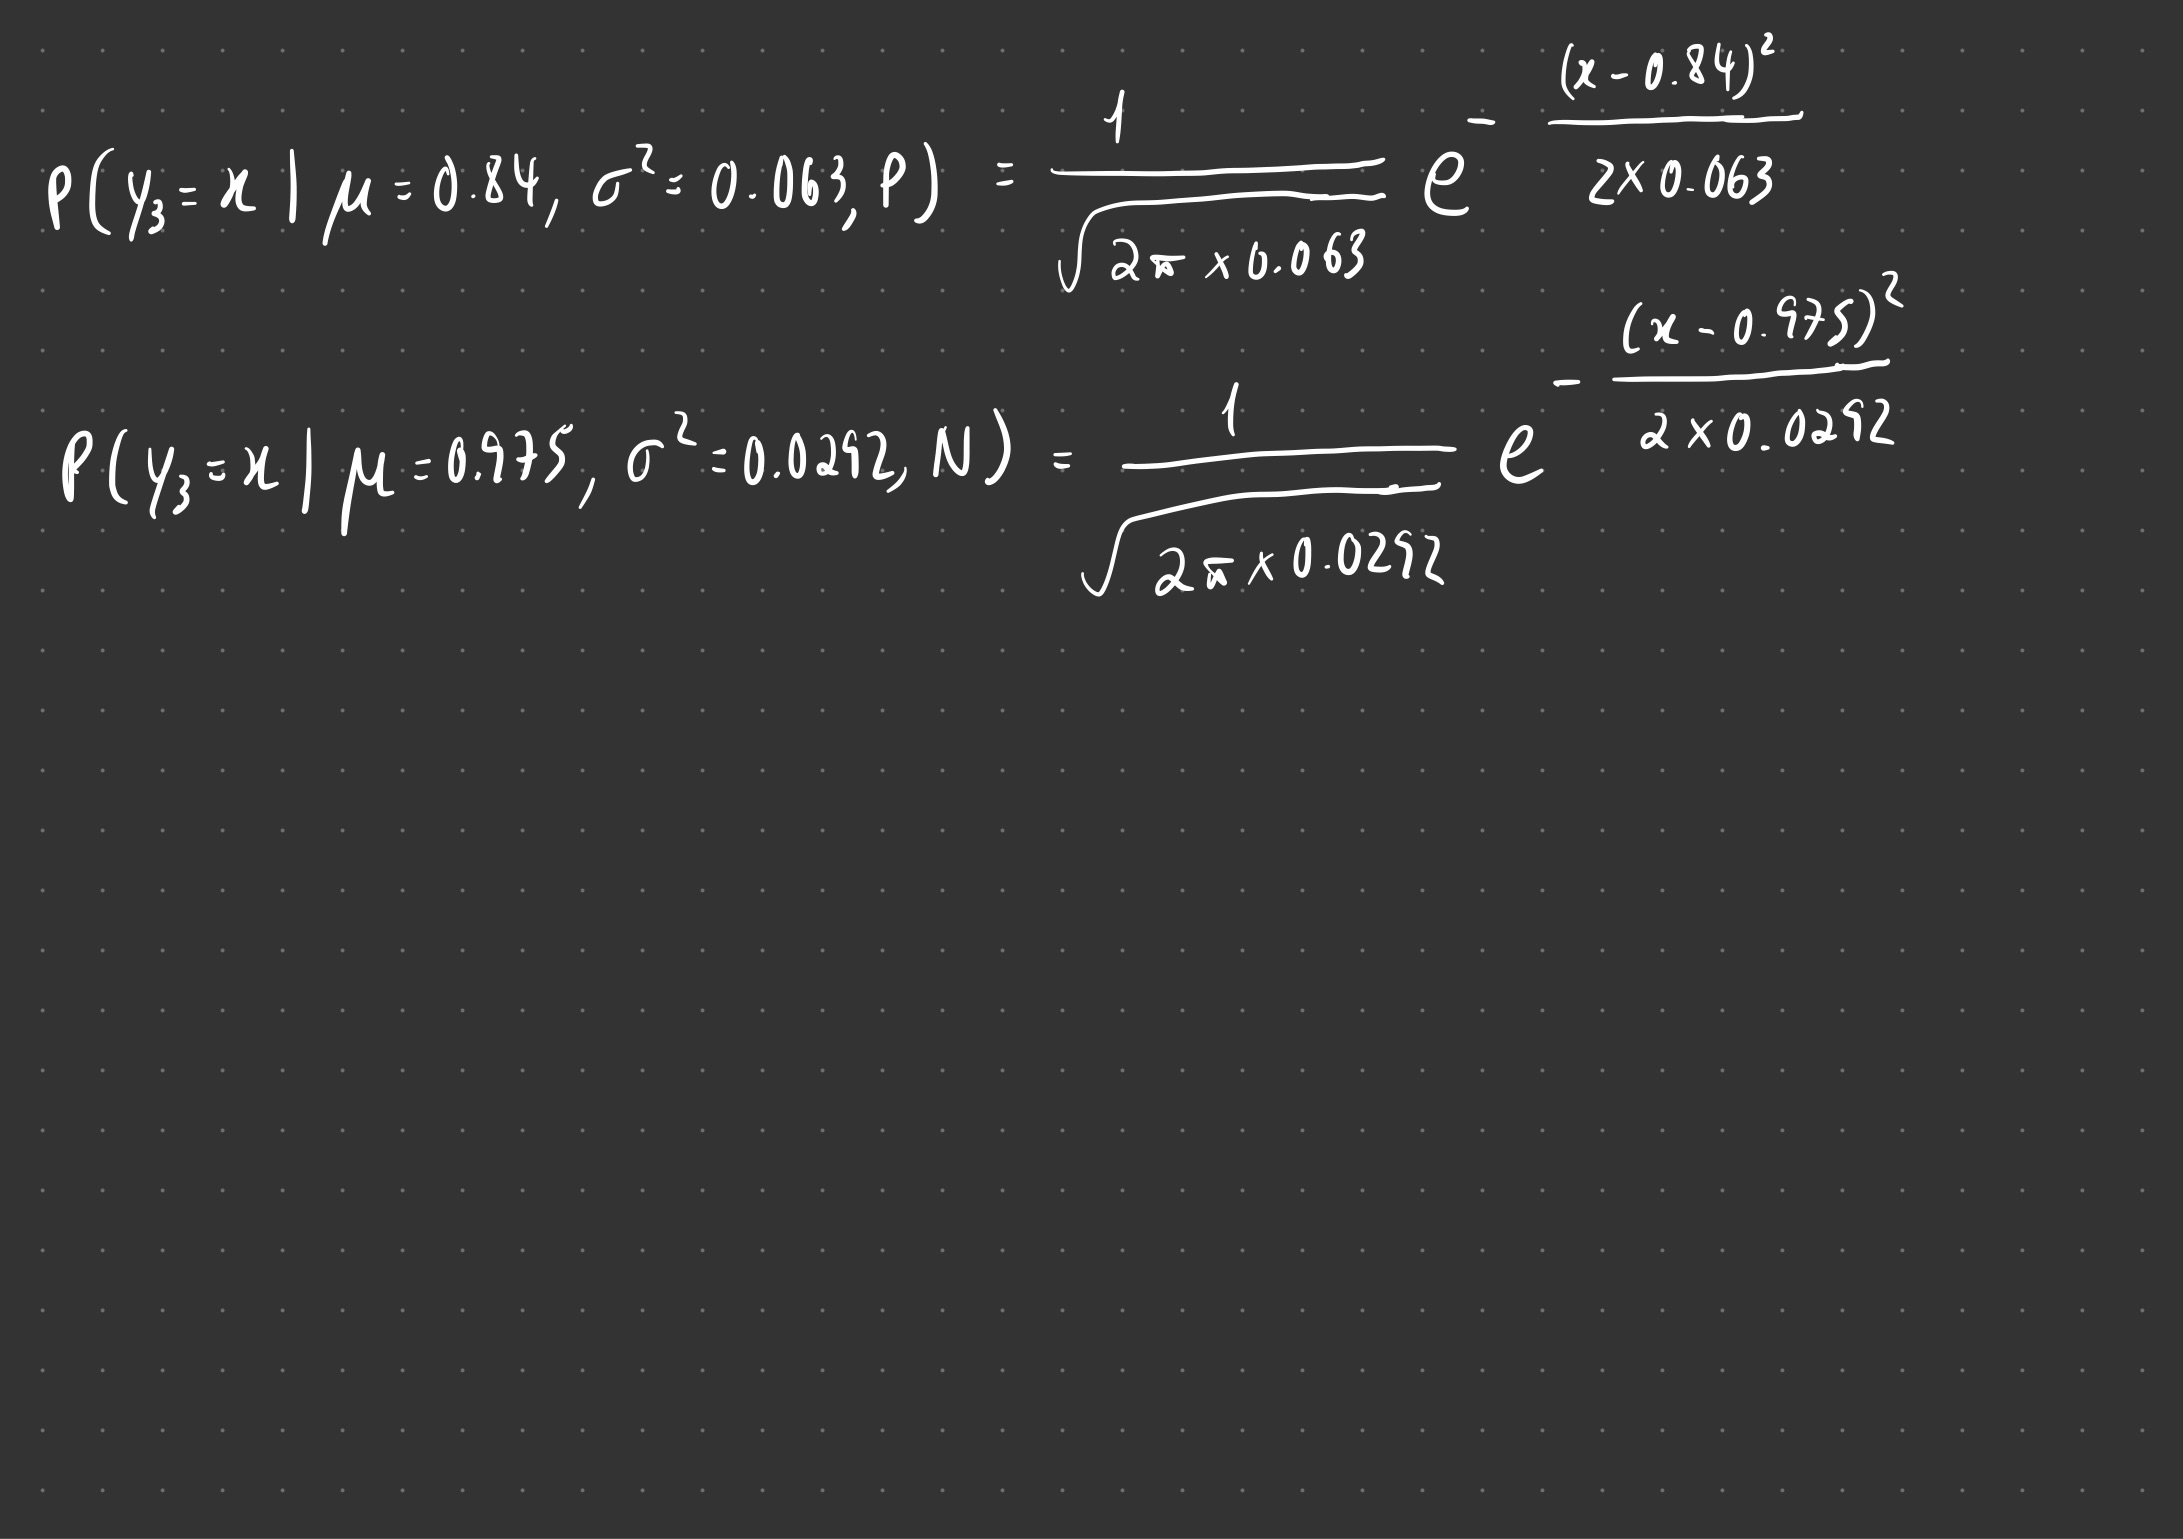
\includegraphics[scale=0.2]{images/Project-15.jpg}
\newline
\end{center}
\newpage
The probability mass function for the Bayesian classifier, the red boxes mean $P(y_1, y_2 | N)$ and the green mean $P(y_1, y_2 | P)$, for $y_1$ and $y_2$ are:
\begin{center}
    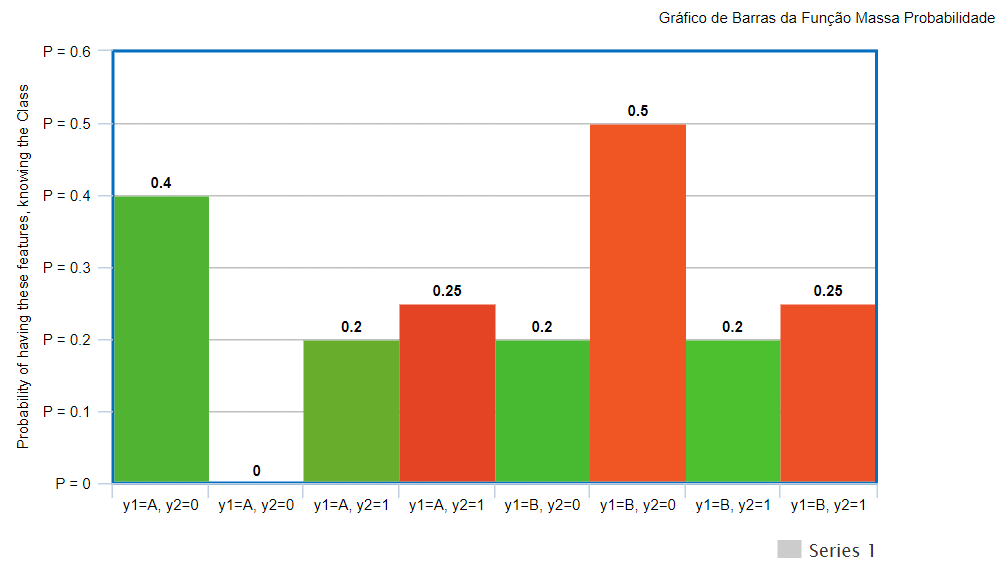
\includegraphics[]{images/graficobarras.png}
\end{center}
The normal distributions of $P(y_3 | P)$ and $P(y_3 | N)$ are, respectively:
\newline
\begin{center}
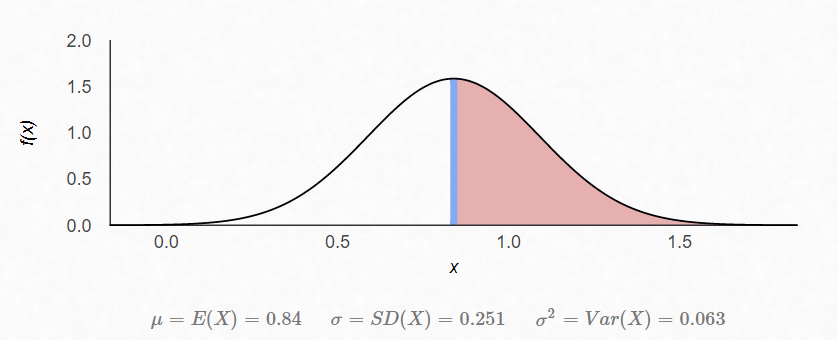
\includegraphics[scale=0.55]{images/positive.png}
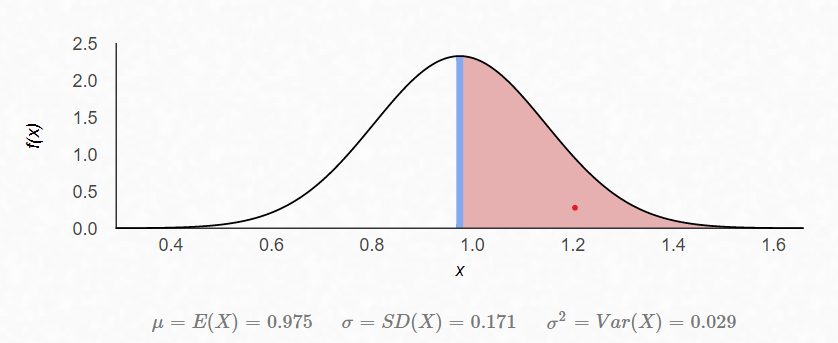
\includegraphics[scale=0.55]{images/negative.png}
\newline
\end{center}
\newpage
\item \leavevmode\vadjust{\vspace{-\baselineskip}}
\begin{center}
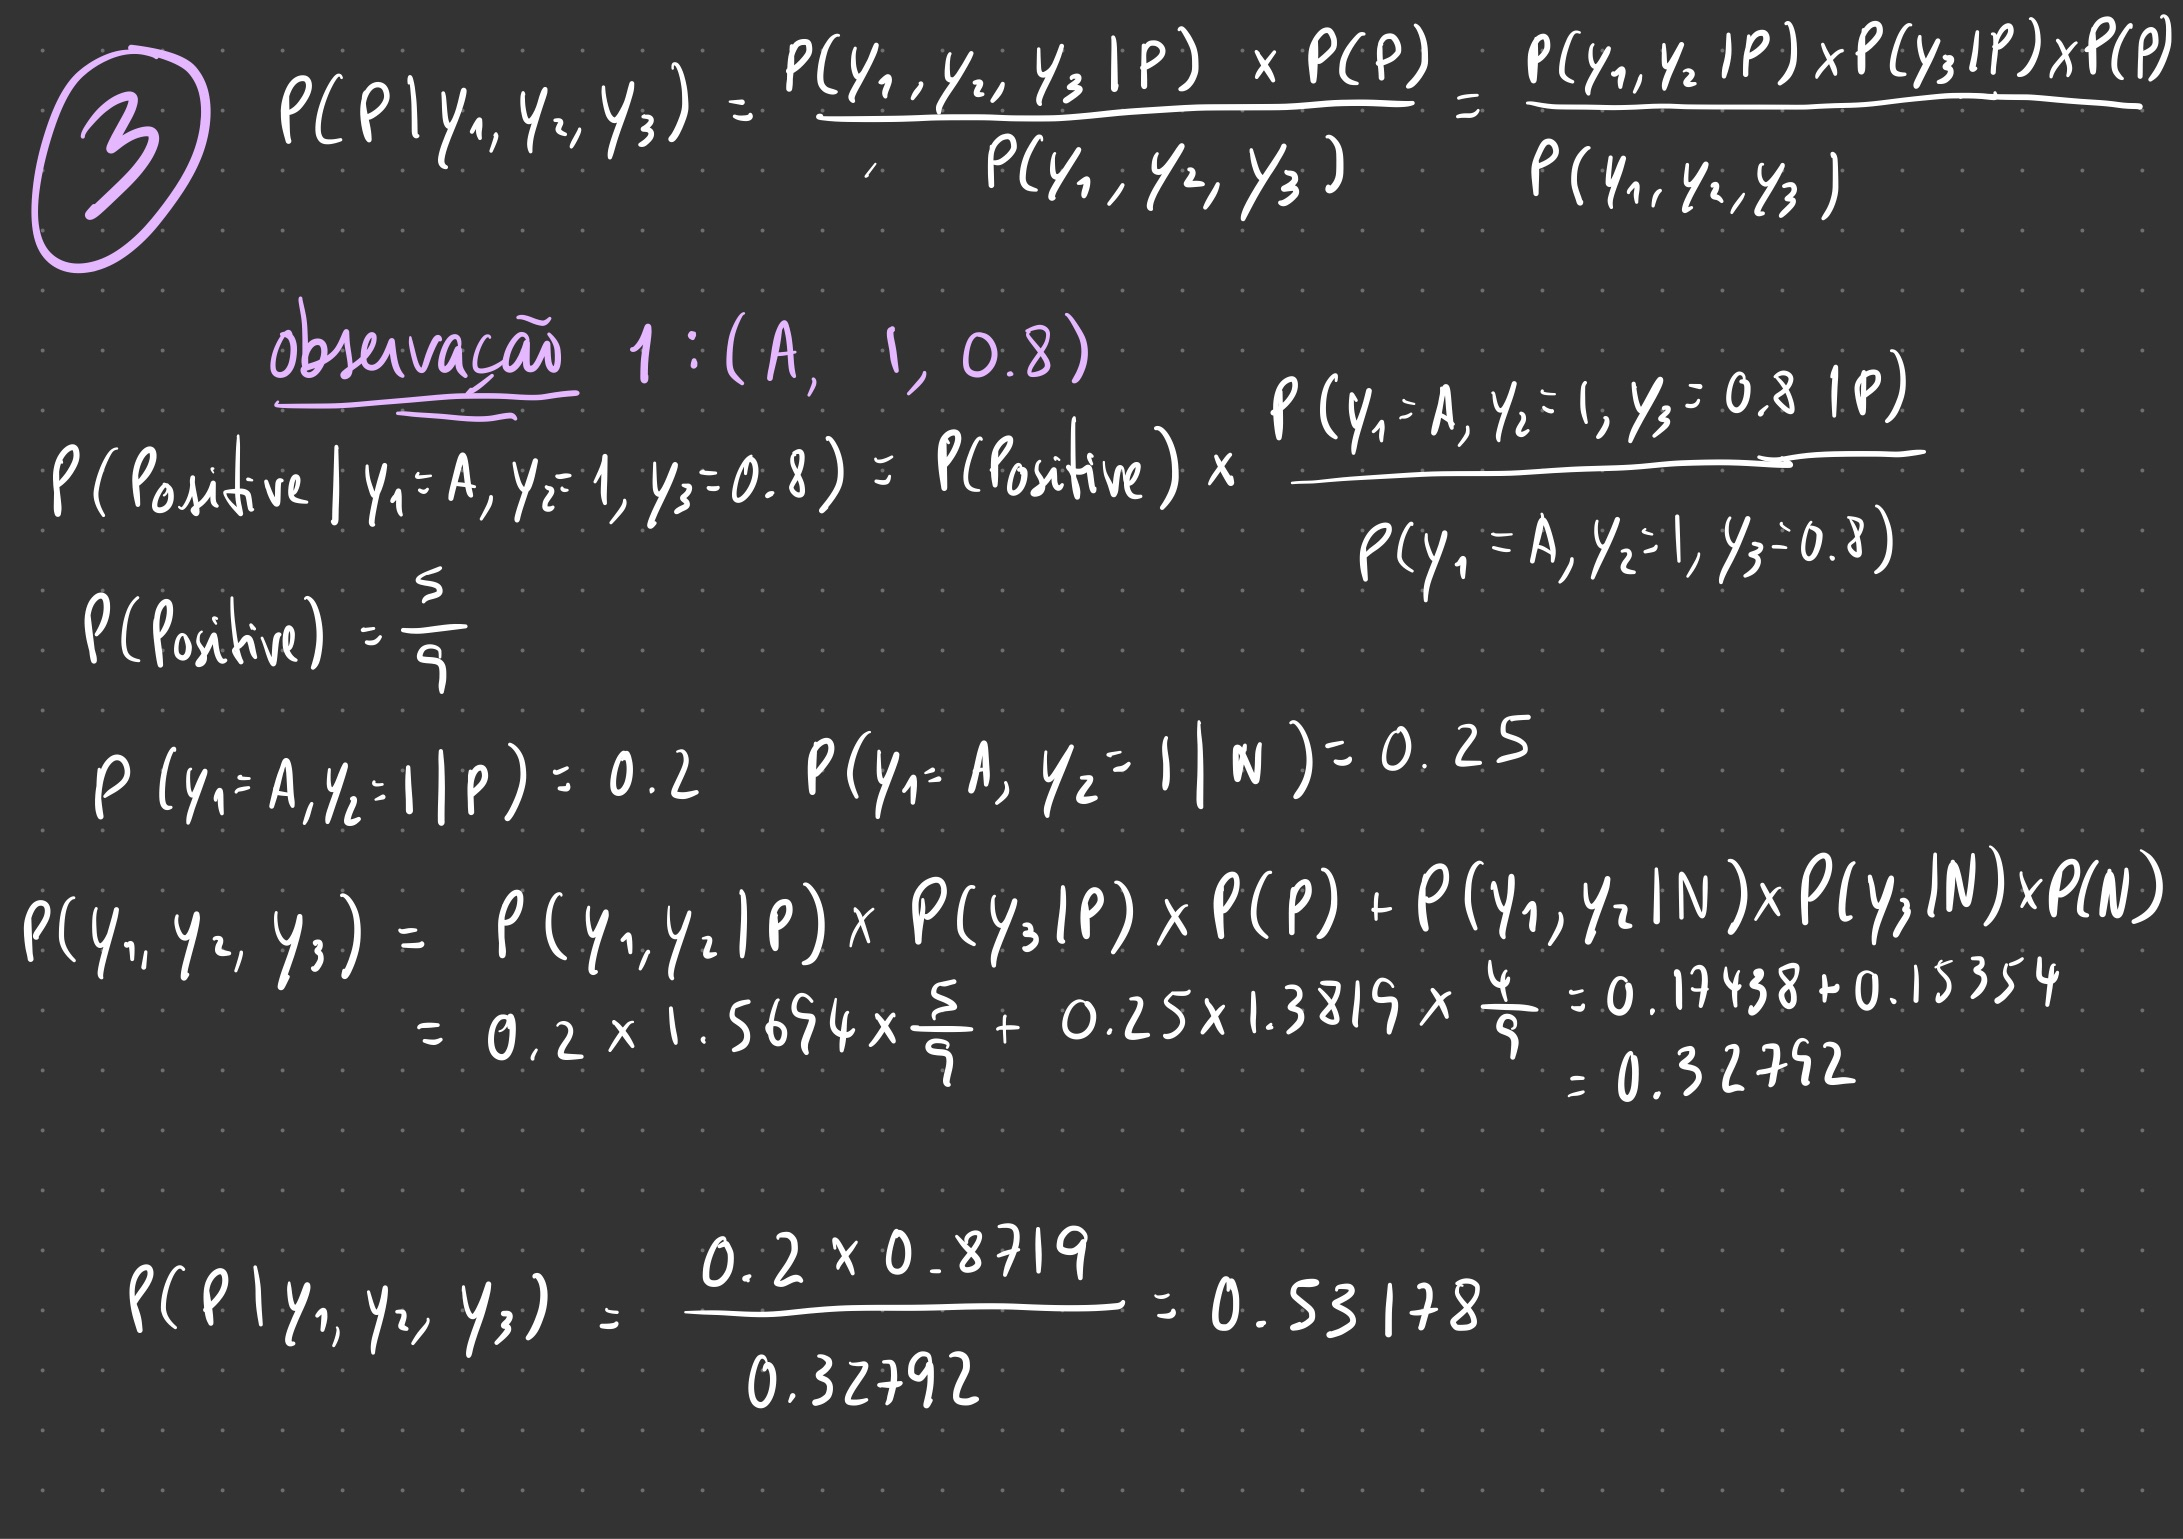
\includegraphics[scale=0.2]{images/Project-16.jpg}
\newline
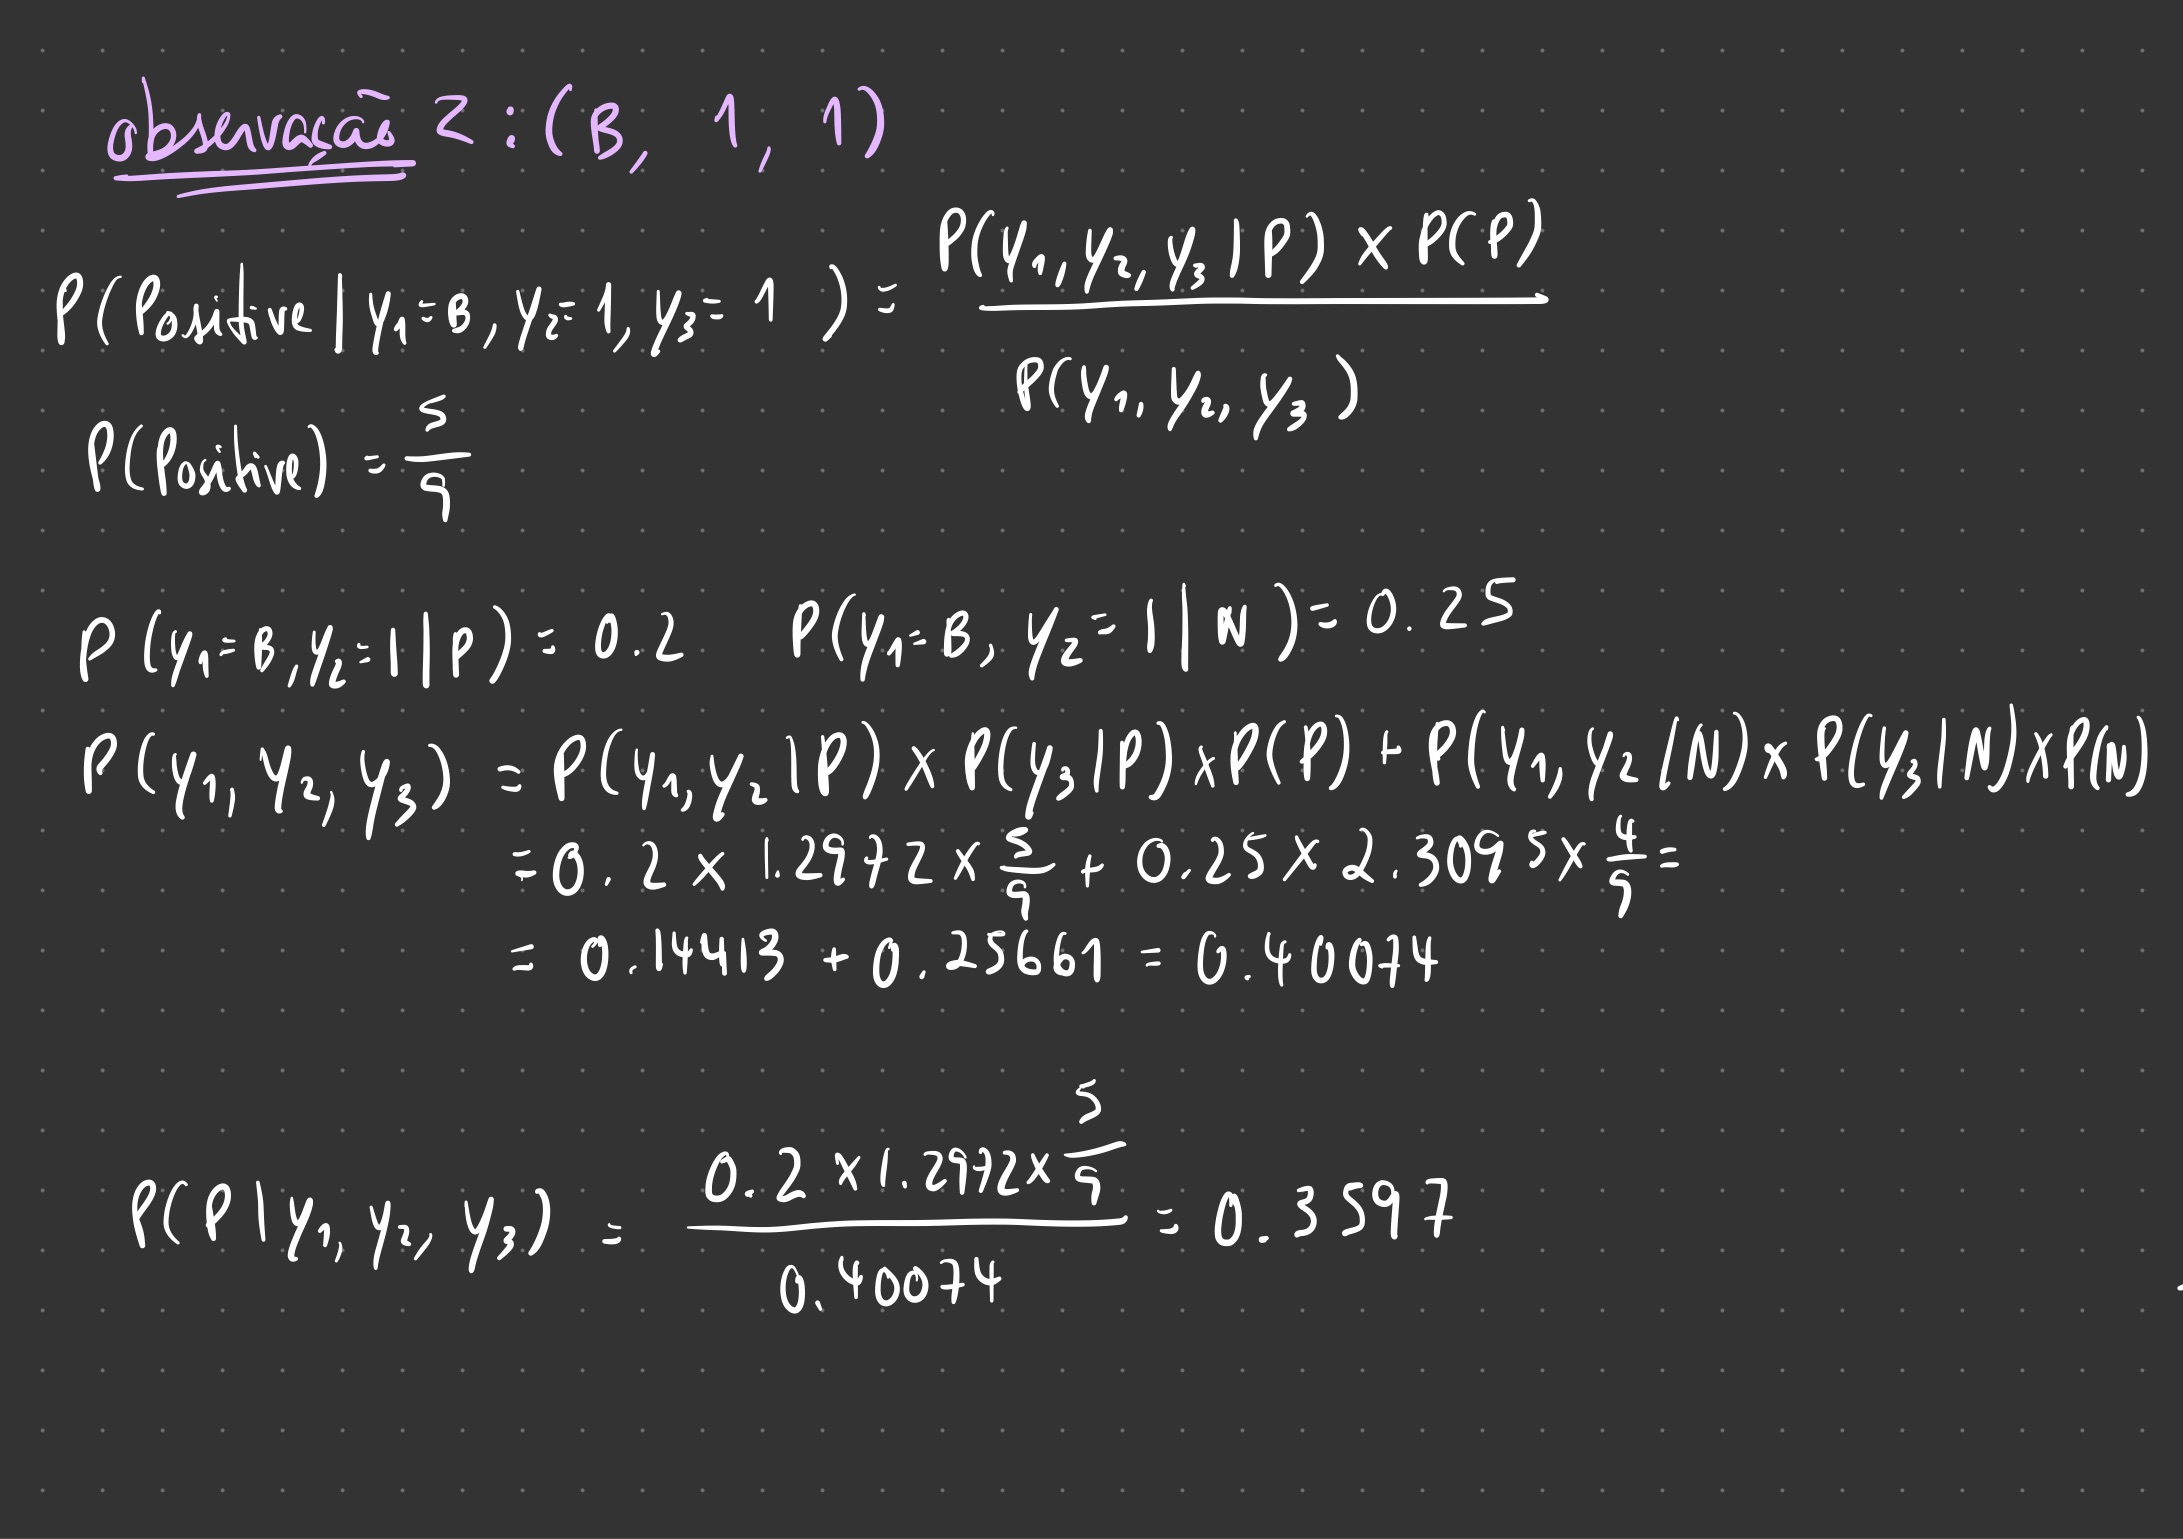
\includegraphics[scale=0.2]{images/Project-17.jpg}
\newline
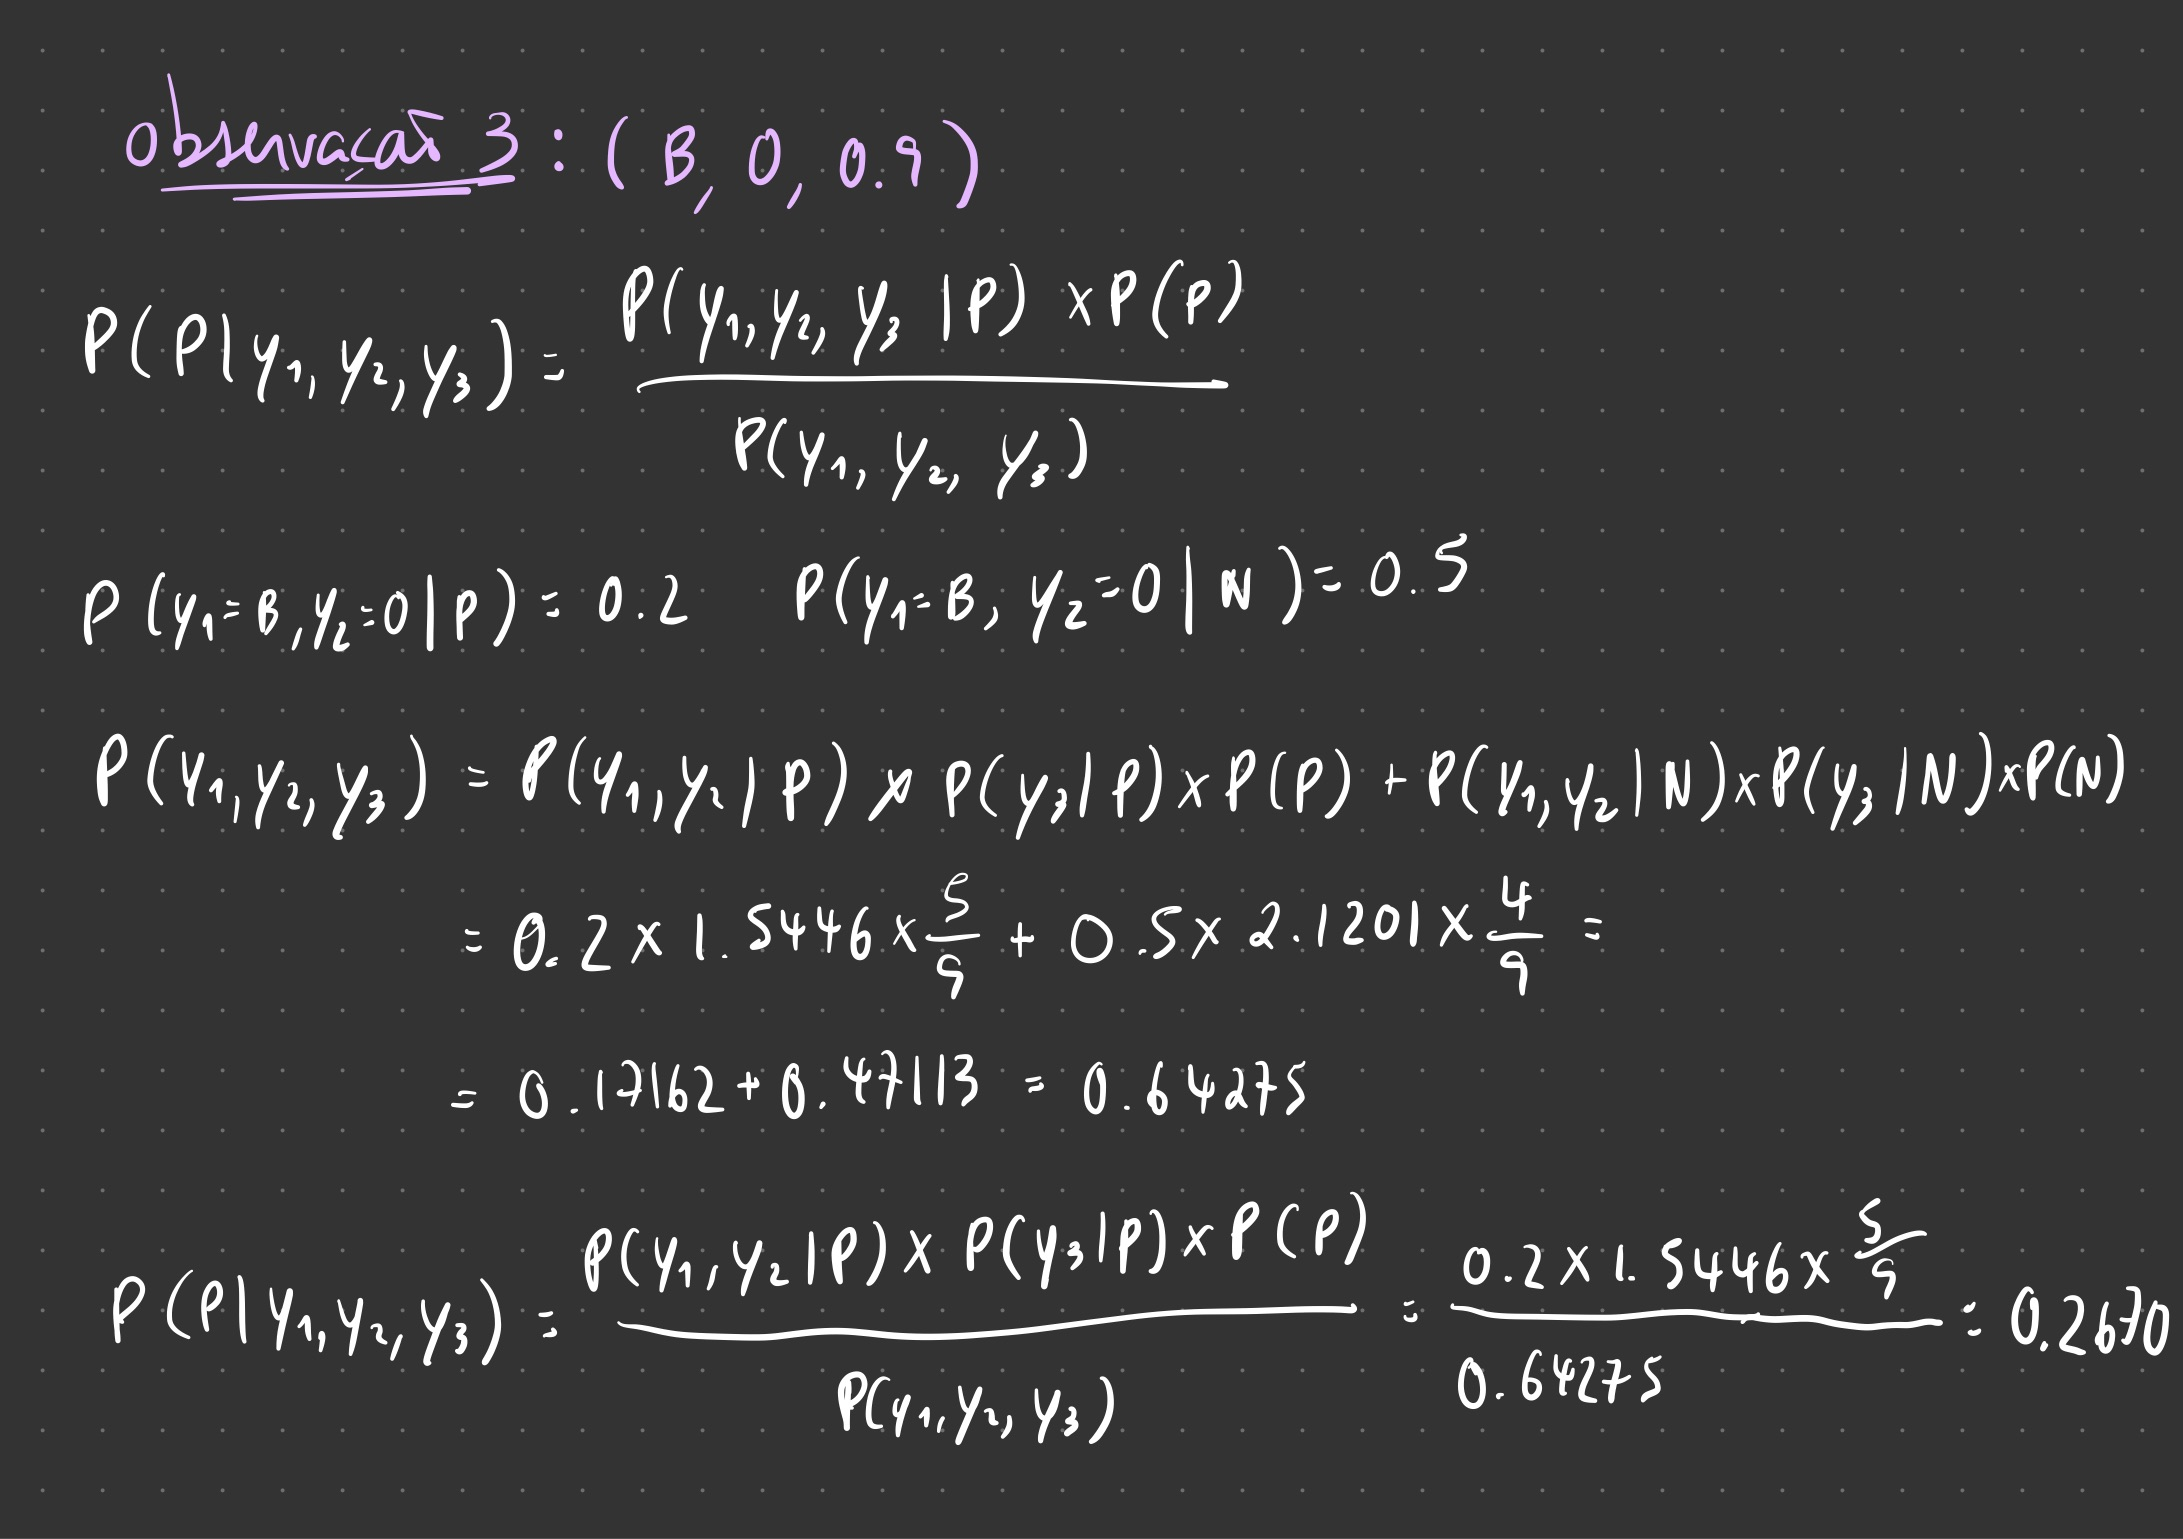
\includegraphics[scale=0.2]{images/Project-18.jpg}
\newline
\end{center}
\item \leavevmode\vadjust{\vspace{-\baselineskip}}
\begin{center}
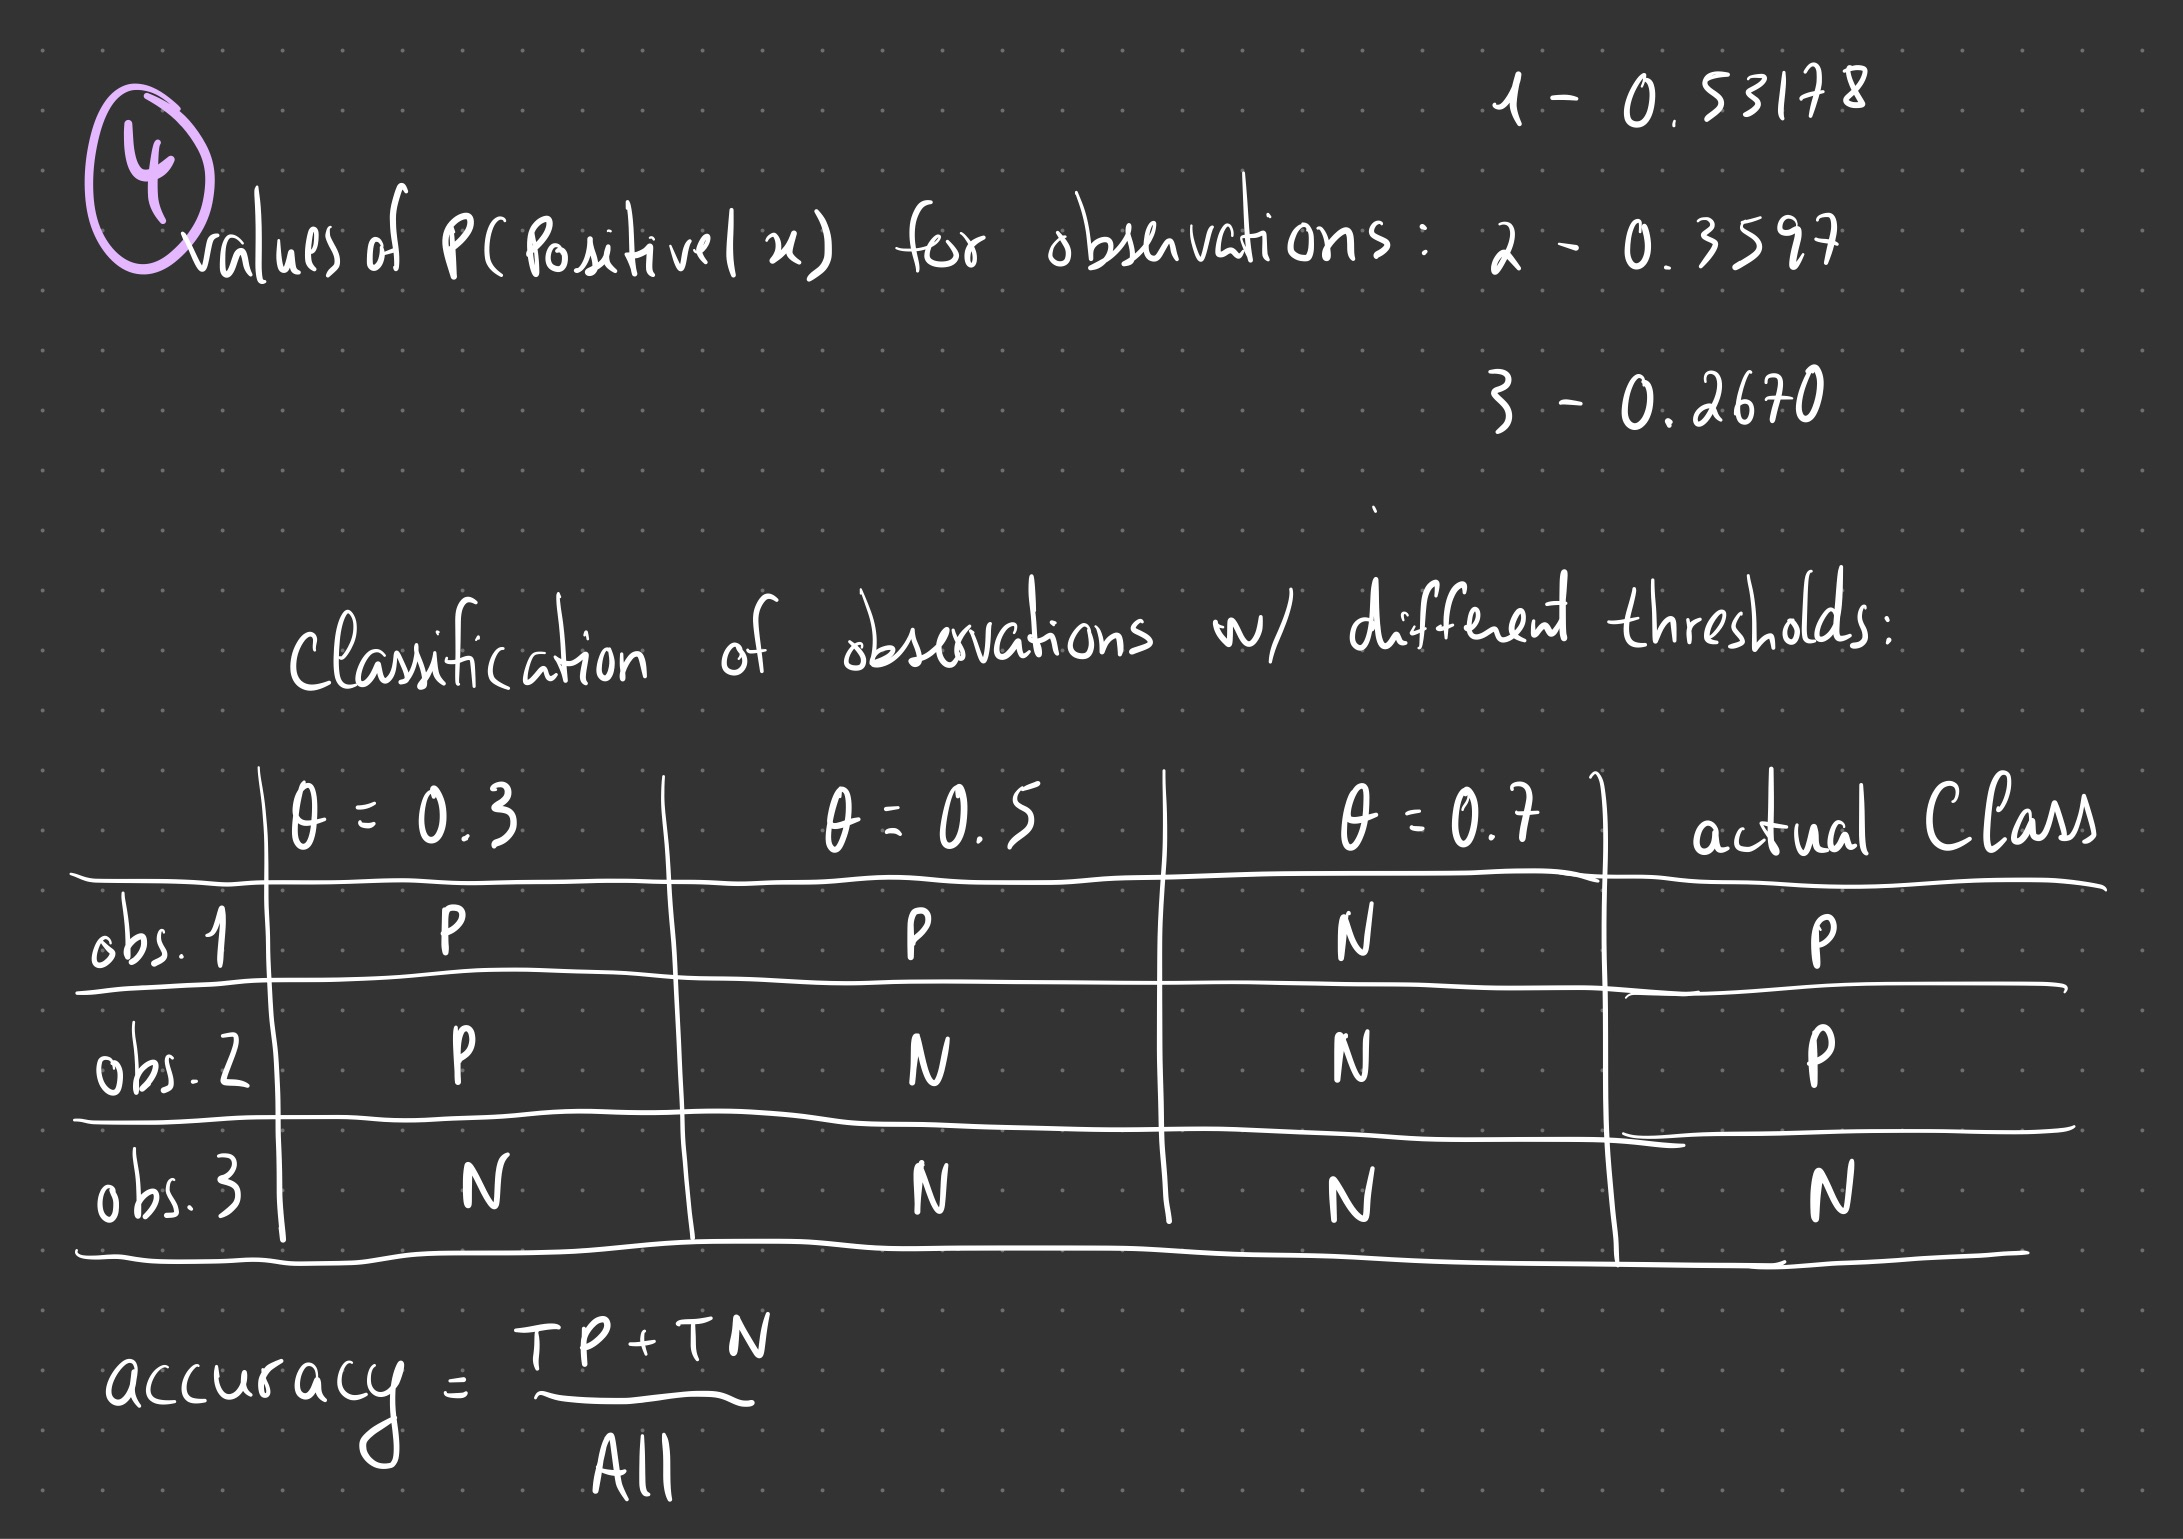
\includegraphics[scale=0.2]{images/Project-19.jpg}
\newline
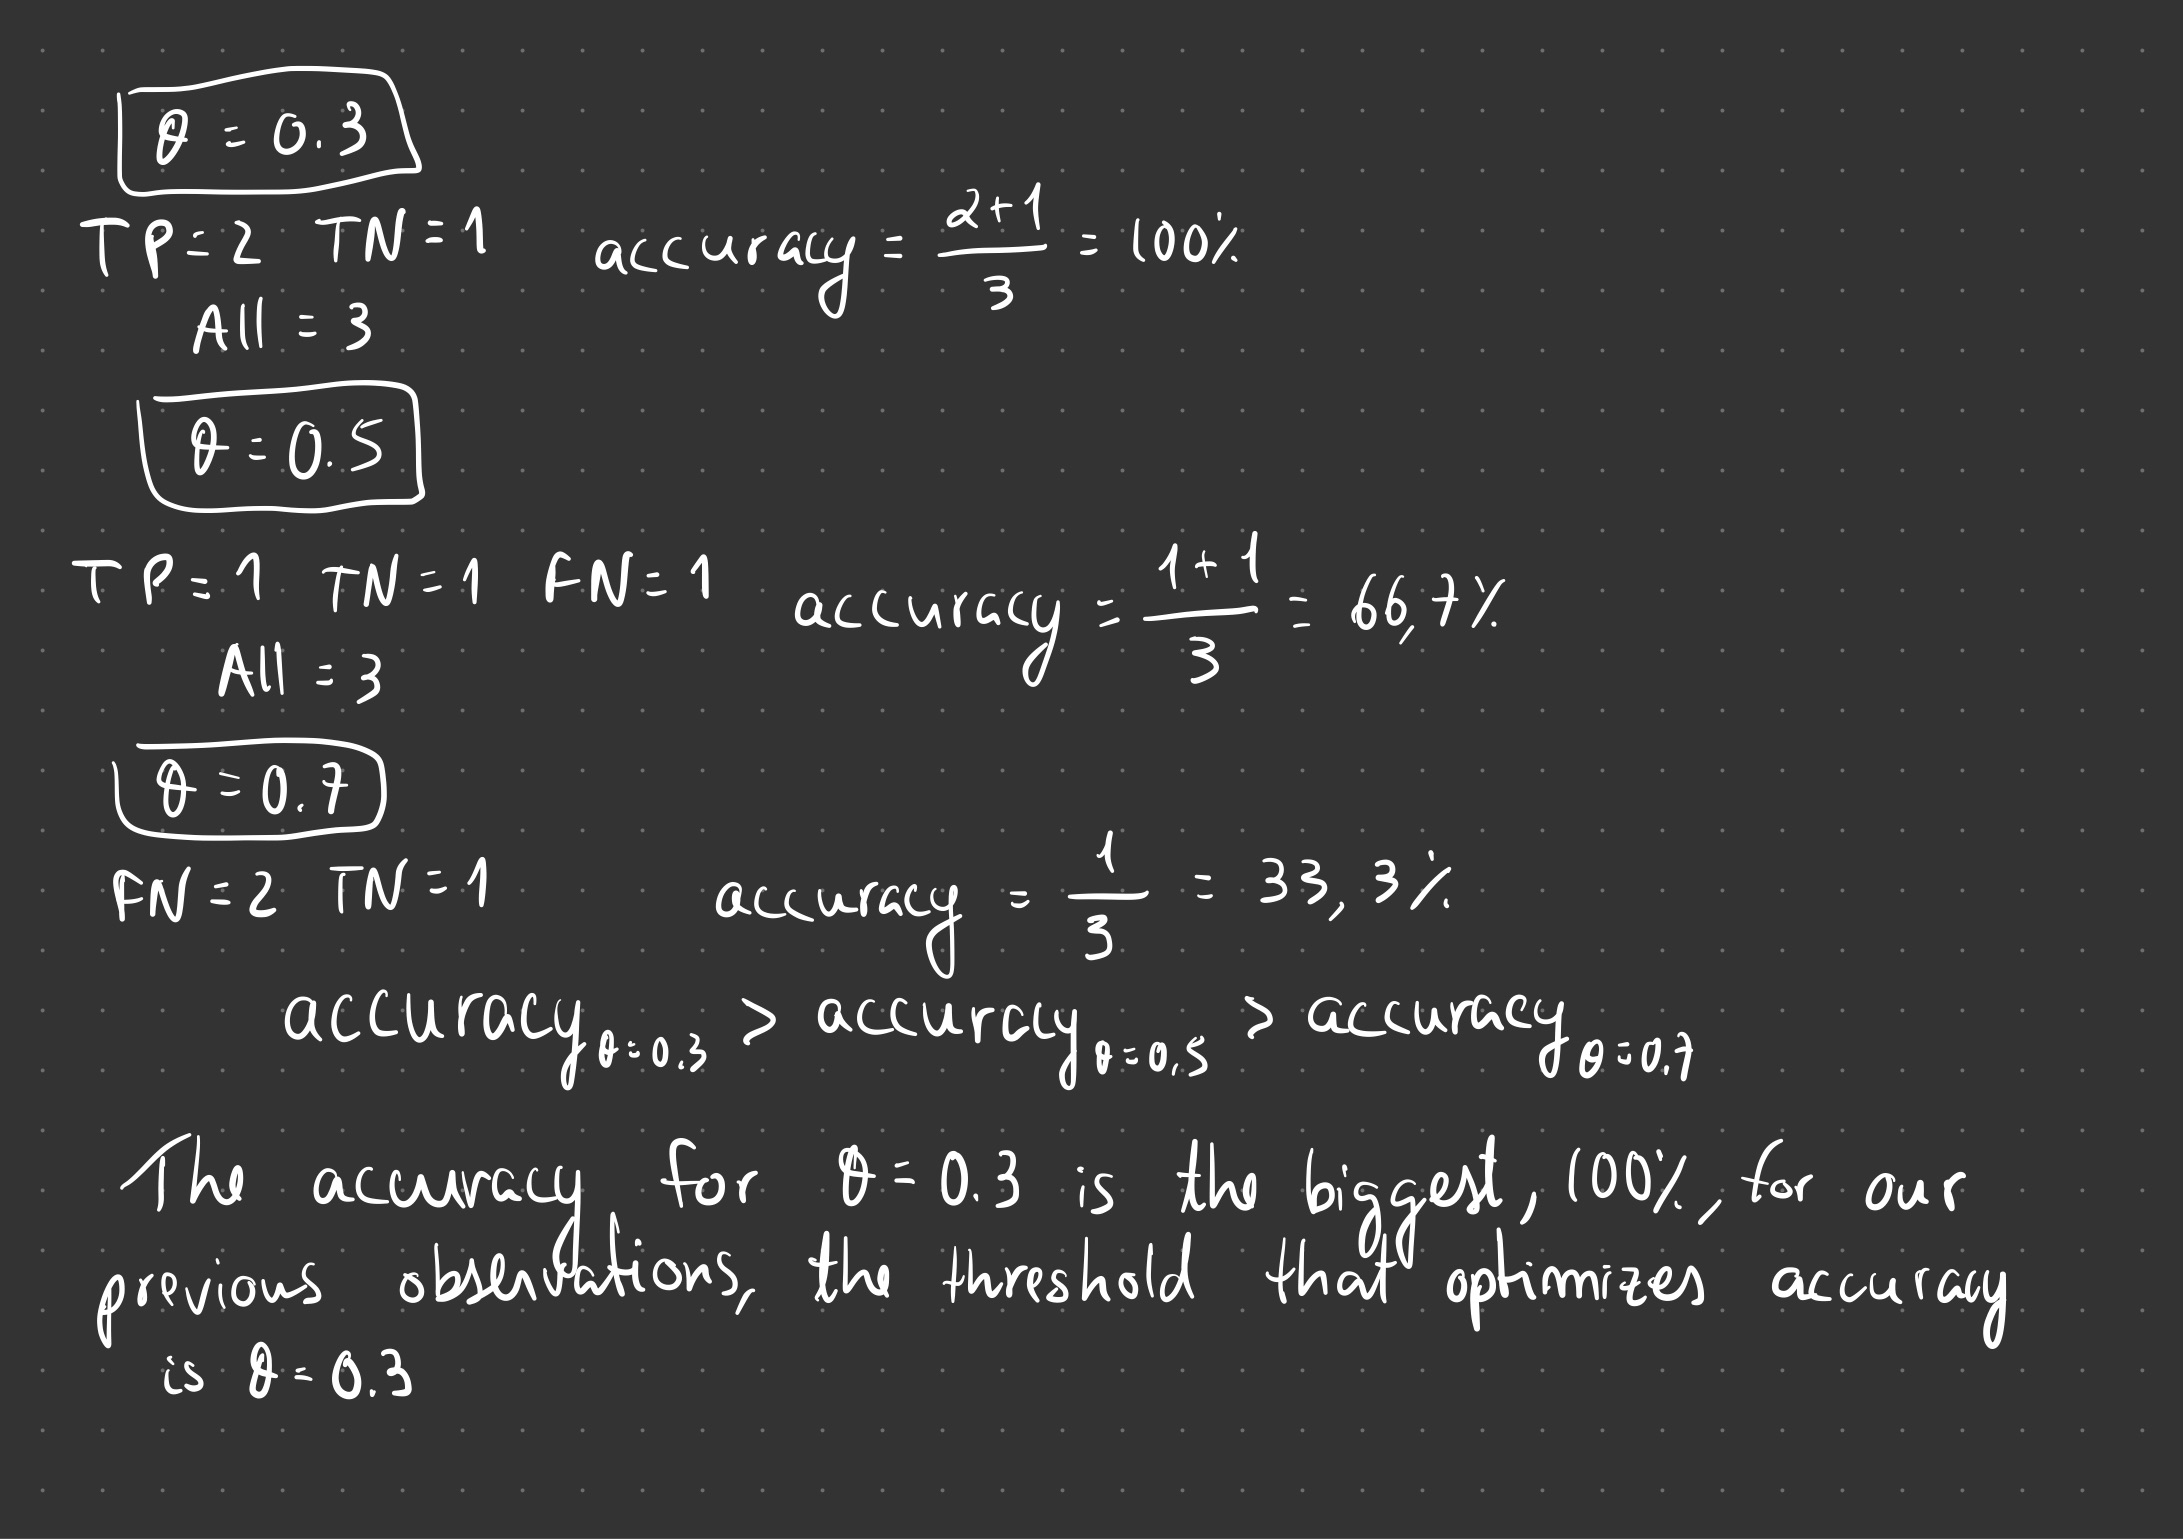
\includegraphics[scale=0.2]{images/Project-20.jpg}
\newline
\end{center}

\end{enumerate}
\newpage
\center\large{\textbf{Part II}: Programming}

\begin{enumerate}[leftmargin=\labelsep,resume]
\item  \leavevmode\vadjust{\vspace{-\baselineskip}}
\begin{center}
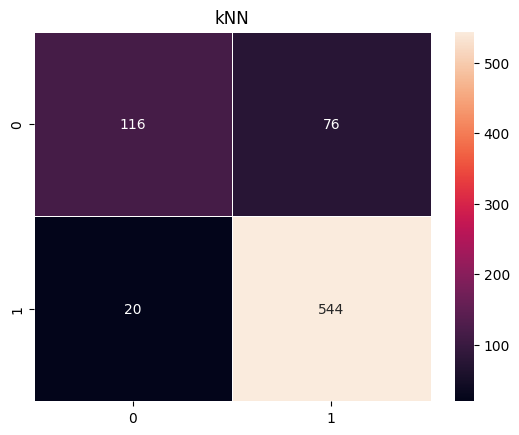
\includegraphics[scale=0.65]{knn}
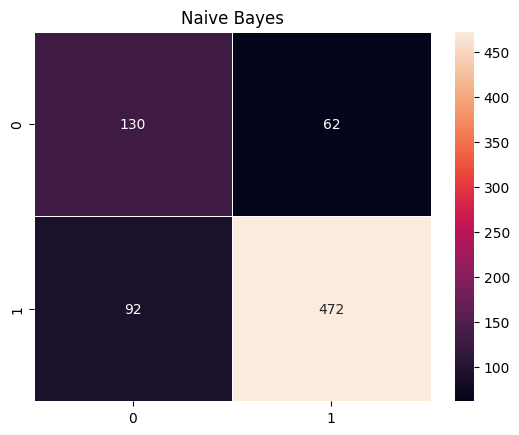
\includegraphics[scale=0.65]{naive}
\end{center}
\item
$knn_{acc}>gnb_{acc}? \ pval= 0.001316817828490826 $\\
$knn_{acc}<gnb_{acc}? \ pval= 0.9986831821715092 $\\
$knn_{acc} \neq gnb_{acc}? \ pval= 0.002633635656981652 $
\newline
\newline
Through the $pval$ we can observe that the accuracy of \textit{k}nn is indeed statistically superior to Naive Bayes' accuracy, with a $pval$ of less than 0.05 ($0.001 < 0.05$), which indicates strong statistical significance, so, our hypothesis is true. 
\item
Since, Naive Bayes is a parametric algorithm, it assumes a functional form, Gaussian distribution in this case, our data set might be non-Gaussian, hence, the poorer performance compared to \textit{k}nn. On a problem that focuses on similarity between observations, \textit{k}nn has an overall better performance due to its nature to locally optimize, although, outliers can worsen its performance significantly, hence, the importance of adjusting \textit{k} to maximise performance.
\end{enumerate}
\newpage
\center\large{\textbf{Appendix}\vskip 0.3cm}

\begin{lstlisting}[language=Python]
import pandas as pd
import seaborn as sns
import matplotlib.pyplot as plt
from scipy import stats
from scipy.io.arff import loadarff
from sklearn.model_selection import StratifiedKFold
from sklearn.neighbors import KNeighborsClassifier
from sklearn.metrics import accuracy_score, confusion_matrix
from sklearn.preprocessing import StandardScaler
from sklearn.naive_bayes import GaussianNB

cm_sum_knn = [[0, 0],[0, 0]]
cm_sum_gnb = [[0, 0],[0, 0]]
knn_acc = []
gnb_acc = []
data = loadarff('pd_speech.arff')
df = pd.DataFrame(data[0])
df['class'] = df['class'].str.decode('utf-8')
X = df.drop('class', axis=1)
y = df['class']

skf = StratifiedKFold(n_splits = 10, shuffle = True, random_state = 0)
knn = KNeighborsClassifier()
gnb = GaussianNB()

for train_index, test_index in skf.split(X, y):
     X_train, X_test, y_train, y_test = X.iloc[train_index], X.iloc[test_index],\
                                        y.iloc[train_index], y.iloc[test_index]
     scaler = StandardScaler().fit(X_train)
     X_train, X_test = scaler.transform(X_train), scaler.transform(X_test)
    

     knn.fit(X_train, y_train)
     y_pred_knn = knn.predict(X_test)
     cm_knn = confusion_matrix(y_test, y_pred_knn)
     knn_acc.append(accuracy_score(y_test, y_pred_knn))

     for i in range(2):
          for j in range(2):
               cm_sum_knn[i][j] += cm_knn[i][j]

     gnb.fit(X_train, y_train)
     y_pred_gnb = gnb.predict(X_test)
     cm_gnb = confusion_matrix(y_test, y_pred_gnb)
     gnb_acc.append(accuracy_score(y_test, y_pred_gnb))

     for i in range(2):
          for j in range(2):
               cm_sum_gnb[i][j] += cm_gnb[i][j]

f, ax = plt.subplots()
sns.heatmap(cm_sum_knn,annot = True, linewidths= 0.5, fmt="g")
plt.title('kNN')
plt.show()

sns.heatmap(cm_sum_gnb,annot = True, linewidths= 0.5, fmt="g")
plt.title('Naive Bayes')
plt.show()

res = stats.ttest_rel(knn_acc, gnb_acc, alternative='greater')
print("knn>gnb? pval=",res.pvalue)

res = stats.ttest_rel(knn_acc, gnb_acc, alternative='less')
print("knn<gnb? pval=",res.pvalue)

res = stats.ttest_rel(knn_acc, gnb_acc, alternative='two-sided')
print("knn!=gnb? pval=",res.pvalue)
\end{lstlisting}

\end{document}